% Options for packages loaded elsewhere
% Options for packages loaded elsewhere
\PassOptionsToPackage{unicode}{hyperref}
\PassOptionsToPackage{hyphens}{url}
\PassOptionsToPackage{dvipsnames,svgnames,x11names}{xcolor}
%
\documentclass[
  letterpaper,
  DIV=11,
  numbers=noendperiod]{scrartcl}
\usepackage{xcolor}
\usepackage{amsmath,amssymb}
\setcounter{secnumdepth}{5}
\usepackage{iftex}
\ifPDFTeX
  \usepackage[T1]{fontenc}
  \usepackage[utf8]{inputenc}
  \usepackage{textcomp} % provide euro and other symbols
\else % if luatex or xetex
  \usepackage{unicode-math} % this also loads fontspec
  \defaultfontfeatures{Scale=MatchLowercase}
  \defaultfontfeatures[\rmfamily]{Ligatures=TeX,Scale=1}
\fi
\usepackage{lmodern}
\ifPDFTeX\else
  % xetex/luatex font selection
\fi
% Use upquote if available, for straight quotes in verbatim environments
\IfFileExists{upquote.sty}{\usepackage{upquote}}{}
\IfFileExists{microtype.sty}{% use microtype if available
  \usepackage[]{microtype}
  \UseMicrotypeSet[protrusion]{basicmath} % disable protrusion for tt fonts
}{}
\makeatletter
\@ifundefined{KOMAClassName}{% if non-KOMA class
  \IfFileExists{parskip.sty}{%
    \usepackage{parskip}
  }{% else
    \setlength{\parindent}{0pt}
    \setlength{\parskip}{6pt plus 2pt minus 1pt}}
}{% if KOMA class
  \KOMAoptions{parskip=half}}
\makeatother
% Make \paragraph and \subparagraph free-standing
\makeatletter
\ifx\paragraph\undefined\else
  \let\oldparagraph\paragraph
  \renewcommand{\paragraph}{
    \@ifstar
      \xxxParagraphStar
      \xxxParagraphNoStar
  }
  \newcommand{\xxxParagraphStar}[1]{\oldparagraph*{#1}\mbox{}}
  \newcommand{\xxxParagraphNoStar}[1]{\oldparagraph{#1}\mbox{}}
\fi
\ifx\subparagraph\undefined\else
  \let\oldsubparagraph\subparagraph
  \renewcommand{\subparagraph}{
    \@ifstar
      \xxxSubParagraphStar
      \xxxSubParagraphNoStar
  }
  \newcommand{\xxxSubParagraphStar}[1]{\oldsubparagraph*{#1}\mbox{}}
  \newcommand{\xxxSubParagraphNoStar}[1]{\oldsubparagraph{#1}\mbox{}}
\fi
\makeatother


\usepackage{longtable,booktabs,array}
\newcounter{none} % for unnumbered tables
\usepackage{calc} % for calculating minipage widths
% Correct order of tables after \paragraph or \subparagraph
\usepackage{etoolbox}
\makeatletter
\patchcmd\longtable{\par}{\if@noskipsec\mbox{}\fi\par}{}{}
\makeatother
% Allow footnotes in longtable head/foot
\IfFileExists{footnotehyper.sty}{\usepackage{footnotehyper}}{\usepackage{footnote}}
\makesavenoteenv{longtable}
\usepackage{graphicx}
\makeatletter
\newsavebox\pandoc@box
\newcommand*\pandocbounded[1]{% scales image to fit in text height/width
  \sbox\pandoc@box{#1}%
  \Gscale@div\@tempa{\textheight}{\dimexpr\ht\pandoc@box+\dp\pandoc@box\relax}%
  \Gscale@div\@tempb{\linewidth}{\wd\pandoc@box}%
  \ifdim\@tempb\p@<\@tempa\p@\let\@tempa\@tempb\fi% select the smaller of both
  \ifdim\@tempa\p@<\p@\scalebox{\@tempa}{\usebox\pandoc@box}%
  \else\usebox{\pandoc@box}%
  \fi%
}
% Set default figure placement to htbp
\def\fps@figure{htbp}
\makeatother





\setlength{\emergencystretch}{3em} % prevent overfull lines

\providecommand{\tightlist}{%
  \setlength{\itemsep}{0pt}\setlength{\parskip}{0pt}}



 


\KOMAoption{captions}{tableheading}
\makeatletter
\@ifpackageloaded{caption}{}{\usepackage{caption}}
\AtBeginDocument{%
\ifdefined\contentsname
  \renewcommand*\contentsname{Table of contents}
\else
  \newcommand\contentsname{Table of contents}
\fi
\ifdefined\listfigurename
  \renewcommand*\listfigurename{List of Figures}
\else
  \newcommand\listfigurename{List of Figures}
\fi
\ifdefined\listtablename
  \renewcommand*\listtablename{List of Tables}
\else
  \newcommand\listtablename{List of Tables}
\fi
\ifdefined\figurename
  \renewcommand*\figurename{Figure}
\else
  \newcommand\figurename{Figure}
\fi
\ifdefined\tablename
  \renewcommand*\tablename{Table}
\else
  \newcommand\tablename{Table}
\fi
}
\@ifpackageloaded{float}{}{\usepackage{float}}
\floatstyle{ruled}
\@ifundefined{c@chapter}{\newfloat{codelisting}{h}{lop}}{\newfloat{codelisting}{h}{lop}[chapter]}
\floatname{codelisting}{Listing}
\newcommand*\listoflistings{\listof{codelisting}{List of Listings}}
\makeatother
\makeatletter
\makeatother
\makeatletter
\@ifpackageloaded{caption}{}{\usepackage{caption}}
\@ifpackageloaded{subcaption}{}{\usepackage{subcaption}}
\makeatother
\usepackage{bookmark}
\IfFileExists{xurl.sty}{\usepackage{xurl}}{} % add URL line breaks if available
\urlstyle{same}
% fallback for those not using the hyperref driver hyperxmp:
\makeatletter
\@ifundefined{xmpquote}{\newcommand{\xmpquote}[1]{#1}}{}
\makeatother
\hypersetup{
  pdftitle={GA4-2: Tracking QA Log},
  pdfauthor={CEP Group 4: Kevin B, Alexa B, Ron S, Brian V},
  colorlinks=true,
  linkcolor={blue},
  filecolor={Maroon},
  citecolor={Blue},
  urlcolor={Blue},
  pdfcreator={LaTeX via pandoc}}


\title{GA4-2: Tracking QA Log}
\usepackage{etoolbox}
\makeatletter
\providecommand{\subtitle}[1]{% add subtitle to \maketitle
  \apptocmd{\@title}{\par {\large #1 \par}}{}{}
}
\makeatother
\subtitle{Wellness Ranch Equine Assisted Therapy}
\author{CEP Group 4: Kevin B, Alexa B, Ron S, Brian V}
\date{2026-10-16}
\begin{document}
\maketitle

\renewcommand*\contentsname{Table of contents}
{
\setcounter{tocdepth}{3}
\tableofcontents
}

\section{Screenshot-Backed QA
Checklist}\label{screenshot-backed-qa-checklist}

\subsection{Testing Overview}\label{testing-overview}

This tracking quality assurance (QA) assessment evaluates the Google
Analytics 4 (GA4) implementation for Wellness Ranch Equine Assisted
Therapy. The purpose is to verify that website interactions are
accurately collected, processed, and reported to support marketing
performance measurement and future analytics activities.

Testing was conducted on October 16, 2026, using the live Wellness Ranch
Therapy website. Google Tag Assistant and GA4 DebugView were used to
verify event collection, trigger behavior, and event parameters. GA4
standard reports were reviewed to assess traffic acquisition, device
categories, page titles, and campaign attribution.

The validation confirmed that page views, user engagement, form
interactions, and lead generation events were received by GA4. Contact
form testing also confirmed that the \texttt{generate\_lead} event was
associated with the website's contact form and contained relevant event
parameters.

Several limitations were identified. The \texttt{generate\_lead} event
was initially not designated as a key event, but this configuration was
updated during testing. Campaign attribution requires further
validation, and the GA4 property does not currently have an active
BigQuery export connection.

The following sections document the validation procedures, supporting
screenshots, observed results, and remaining limitations.

\subsection{GTM / Collection Layer}\label{gtm-collection-layer}

\subsubsection{Collection Layer
Validation}\label{collection-layer-validation}

Google Tag Assistant was used on October 16, 2026, to verify that the
Google tag was installed and sending events from the live Wellness Ranch
Therapy website.

The testing confirmed that the website was connected to Google Tag
Assistant and that the Google tag with measurement ID
\texttt{G-FL3S97QPD6} was detected.

The Tag Assistant results also showed that page views, user engagement,
form interactions, and lead generation events were being transmitted to
GA4.

\subsubsection{Tag Assistant Connection}\label{tag-assistant-connection}

\begin{figure}[H]

{\centering \pandocbounded{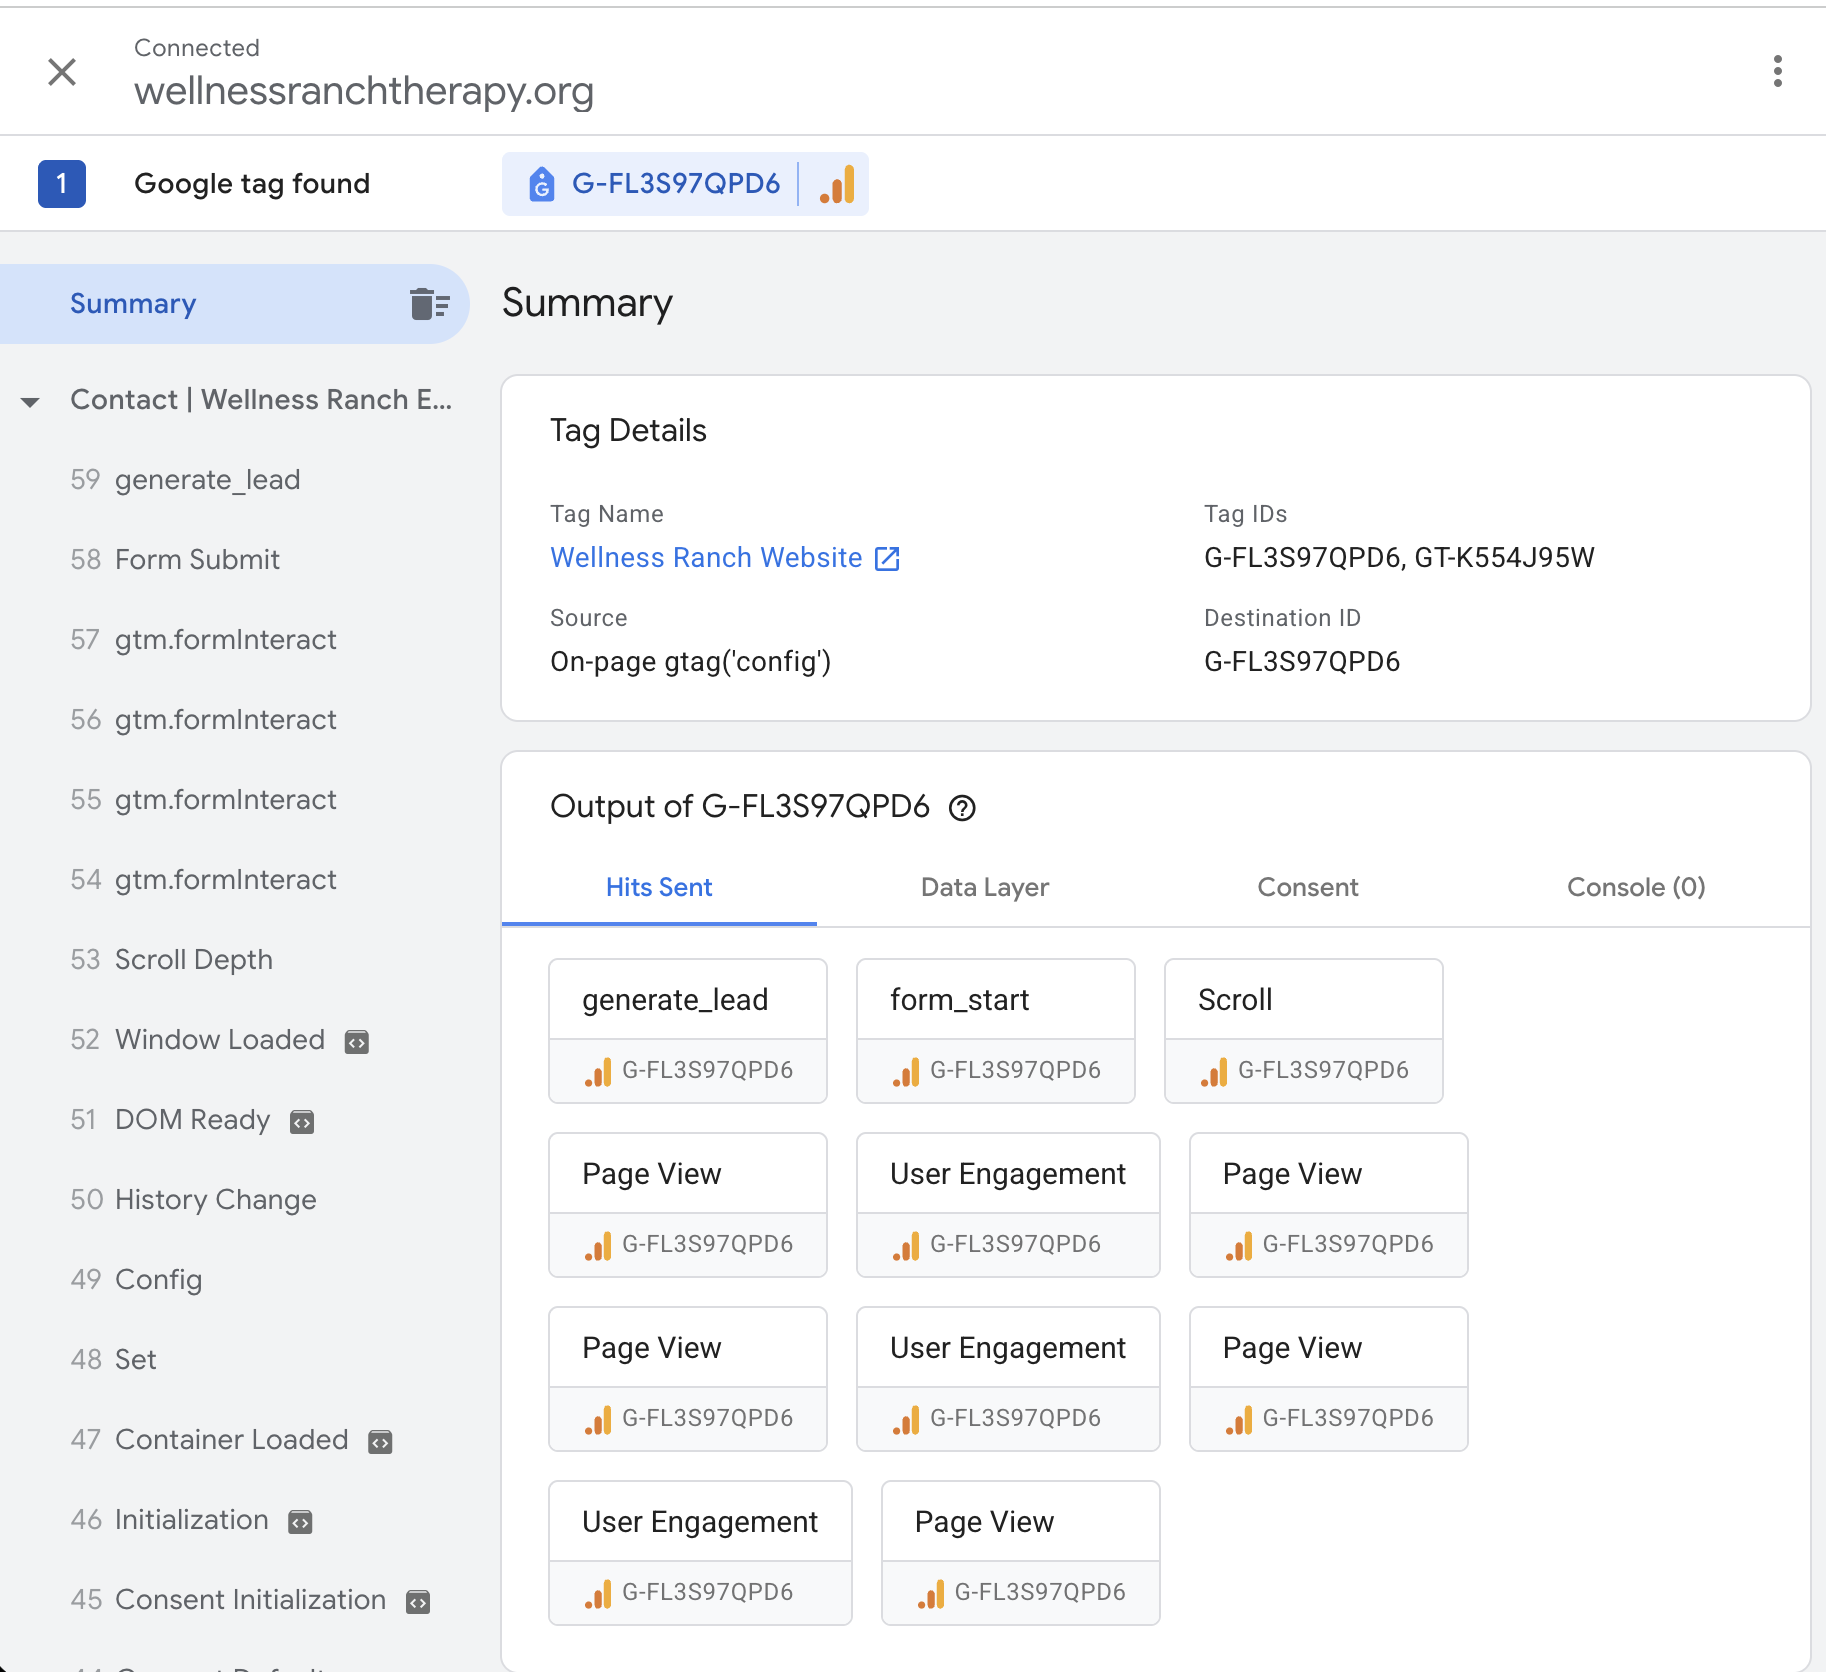
\includegraphics[keepaspectratio]{images/TagAssistant_Connection.png}}

}

\caption{Google Tag Assistant connection and detected Google tag}

\end{figure}%

\subsubsection{Lead Event Validation}\label{lead-event-validation}

A test contact form submission generated a \texttt{generate\_lead}
event. Tag Assistant showed one \texttt{generate\_lead} hit sent to the
GA4 measurement ID during the selected submission event.

\begin{figure}[H]

{\centering \pandocbounded{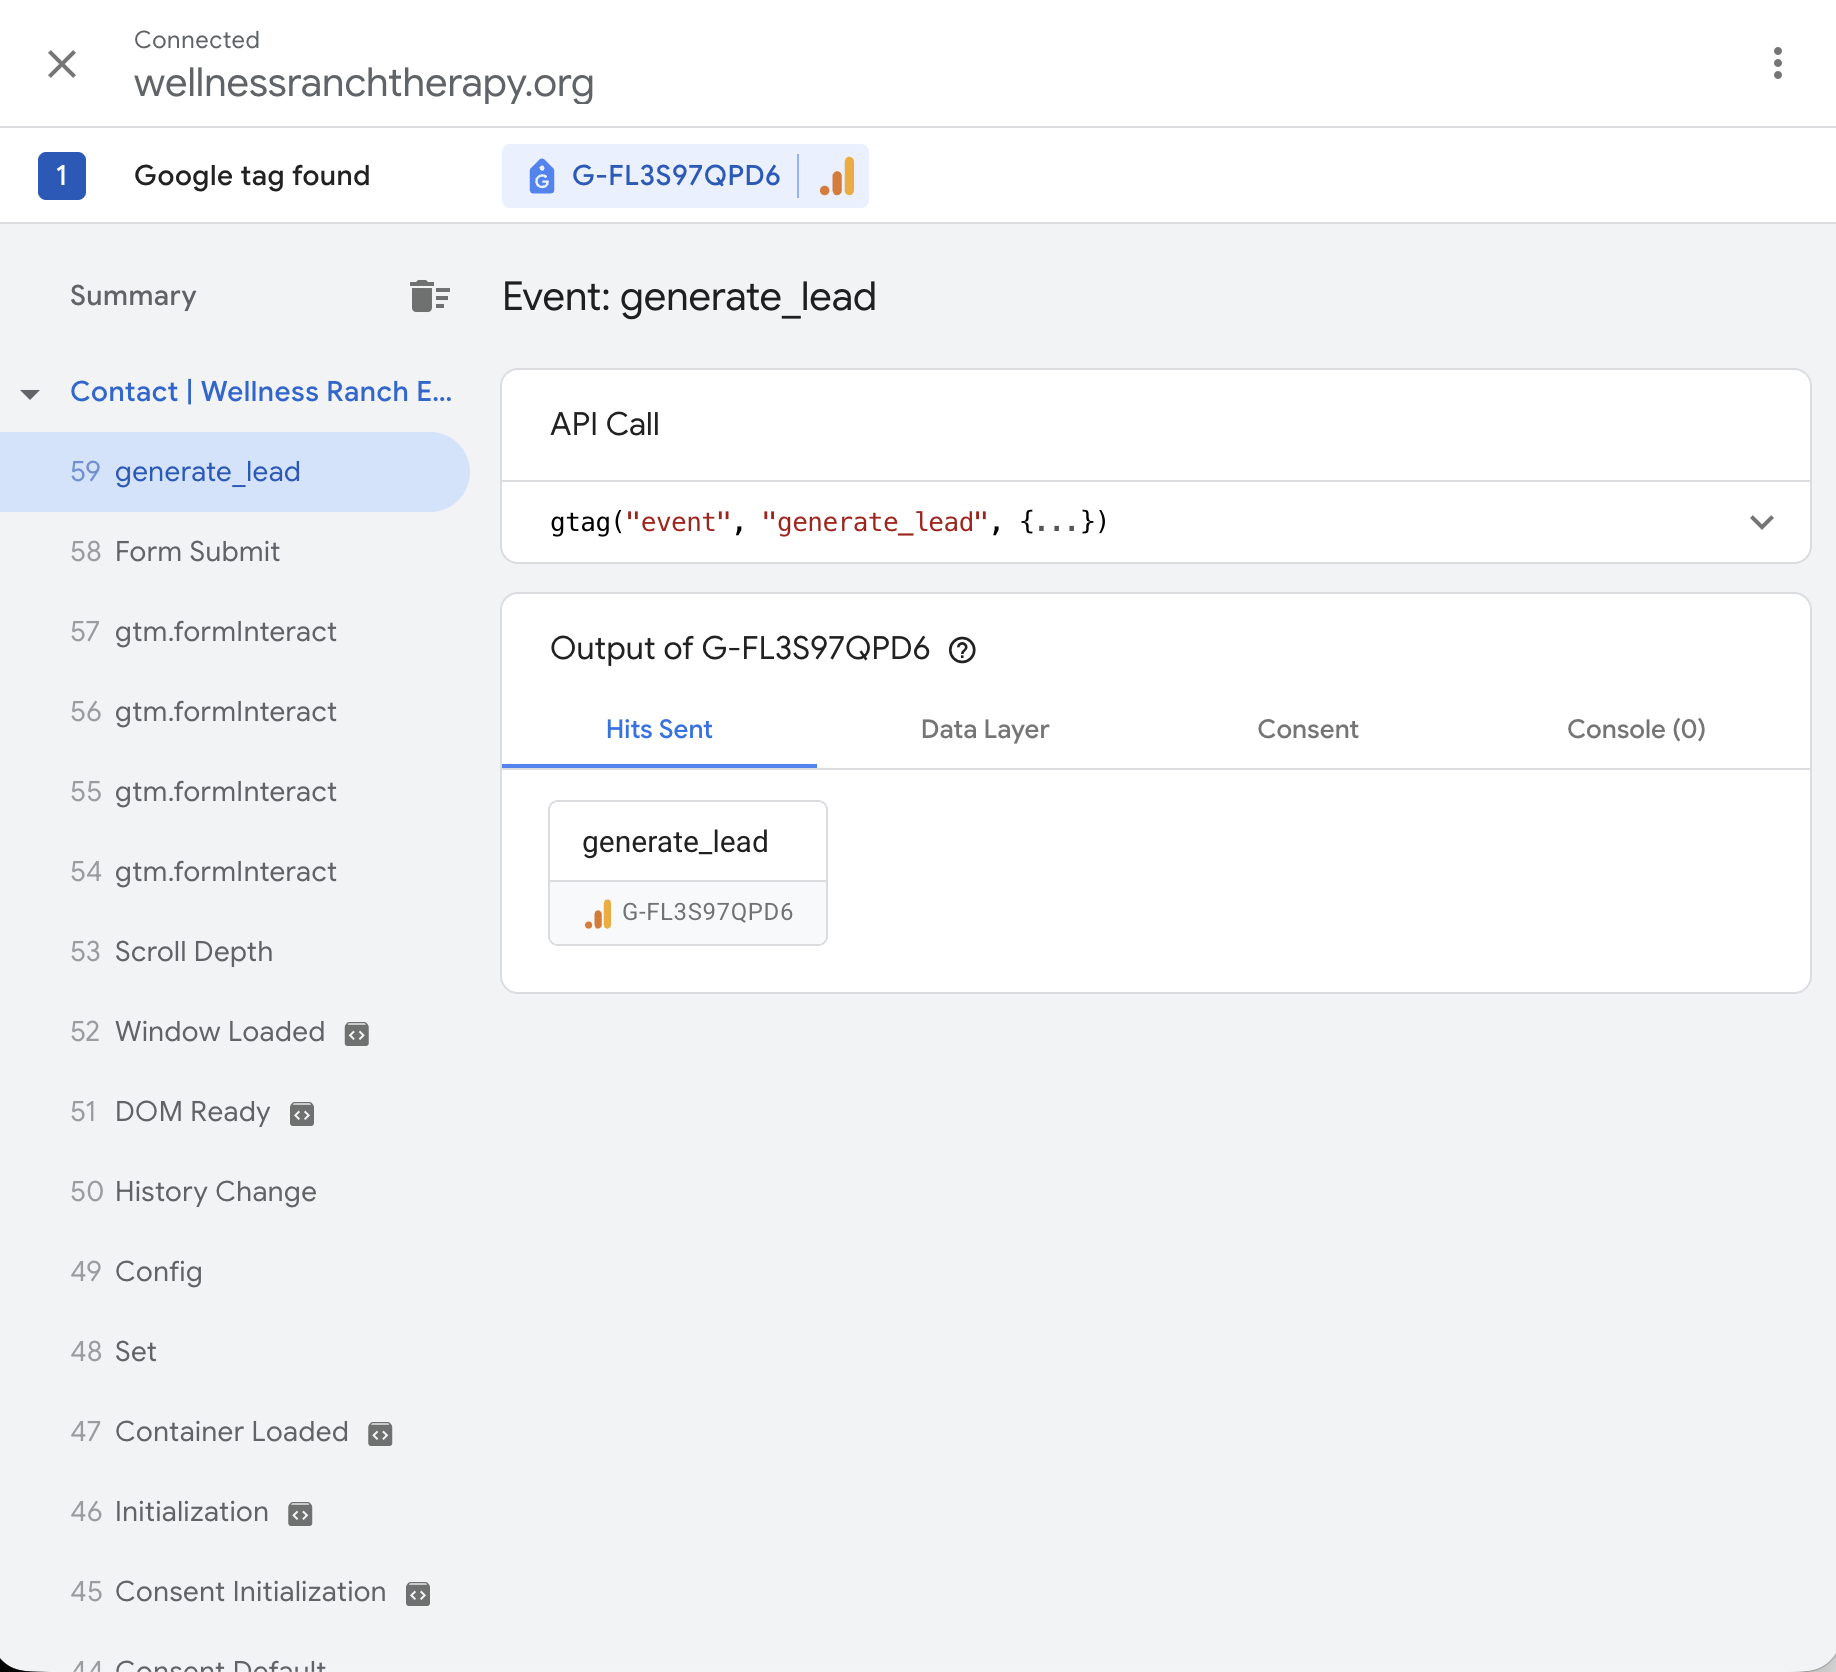
\includegraphics[keepaspectratio]{images/TagAssistant_GenerateLead.png}}

}

\caption{Tag Assistant generate\_lead event validation}

\end{figure}%

\subsubsection{QA Results}\label{qa-results}

{\def\LTcaptype{none} % do not increment counter
\begin{longtable}[]{@{}
  >{\raggedright\arraybackslash}p{(\linewidth - 6\tabcolsep) * \real{0.2500}}
  >{\raggedright\arraybackslash}p{(\linewidth - 6\tabcolsep) * \real{0.2500}}
  >{\raggedright\arraybackslash}p{(\linewidth - 6\tabcolsep) * \real{0.2500}}
  >{\raggedright\arraybackslash}p{(\linewidth - 6\tabcolsep) * \real{0.2500}}@{}}
\toprule\noalign{}
\begin{minipage}[b]{\linewidth}\raggedright
Test
\end{minipage} & \begin{minipage}[b]{\linewidth}\raggedright
Expected Result
\end{minipage} & \begin{minipage}[b]{\linewidth}\raggedright
Observed Result
\end{minipage} & \begin{minipage}[b]{\linewidth}\raggedright
Status
\end{minipage} \\
\midrule\noalign{}
\endhead
\bottomrule\noalign{}
\endlastfoot
Google tag installation & Correct tag detected & G-FL3S97QPD6 detected &
Pass \\
Page view tracking & Page views sent to GA4 & Page view hits observed &
Pass \\
Form interaction tracking & Form start event sent & form\_start observed
& Pass \\
Lead generation tracking & generate\_lead sent after submission & One
lead hit observed & Pass \\
Duplicate lead tracking & One event per submission & One hit observed in
selected test & Pass (limited test) \\
\end{longtable}
}

The collection-layer tests confirmed that the Google tag was sending the
expected events. However, additional testing across multiple submissions
and devices is recommended to rule out intermittent duplicate events.

\subsection{GA4 DebugView and Realtime
Validation}\label{ga4-debugview-and-realtime-validation}

After confirming the Google tag was sending events in Tag Assistant, we
checked that those events were actually being received and processed in
GA4. We turned on debug mode, browsed the live Wellness Ranch site, and
reviewed the results in two places: DebugView (Admin → Data display →
DebugView) and the Realtime overview. For each event, we checked three
things: did it show up, were the parameters filled in, and did the
values make sense.

\subsubsection{Do the events show up in
DebugView?}\label{do-the-events-show-up-in-debugview}

\begin{figure}[H]

{\centering 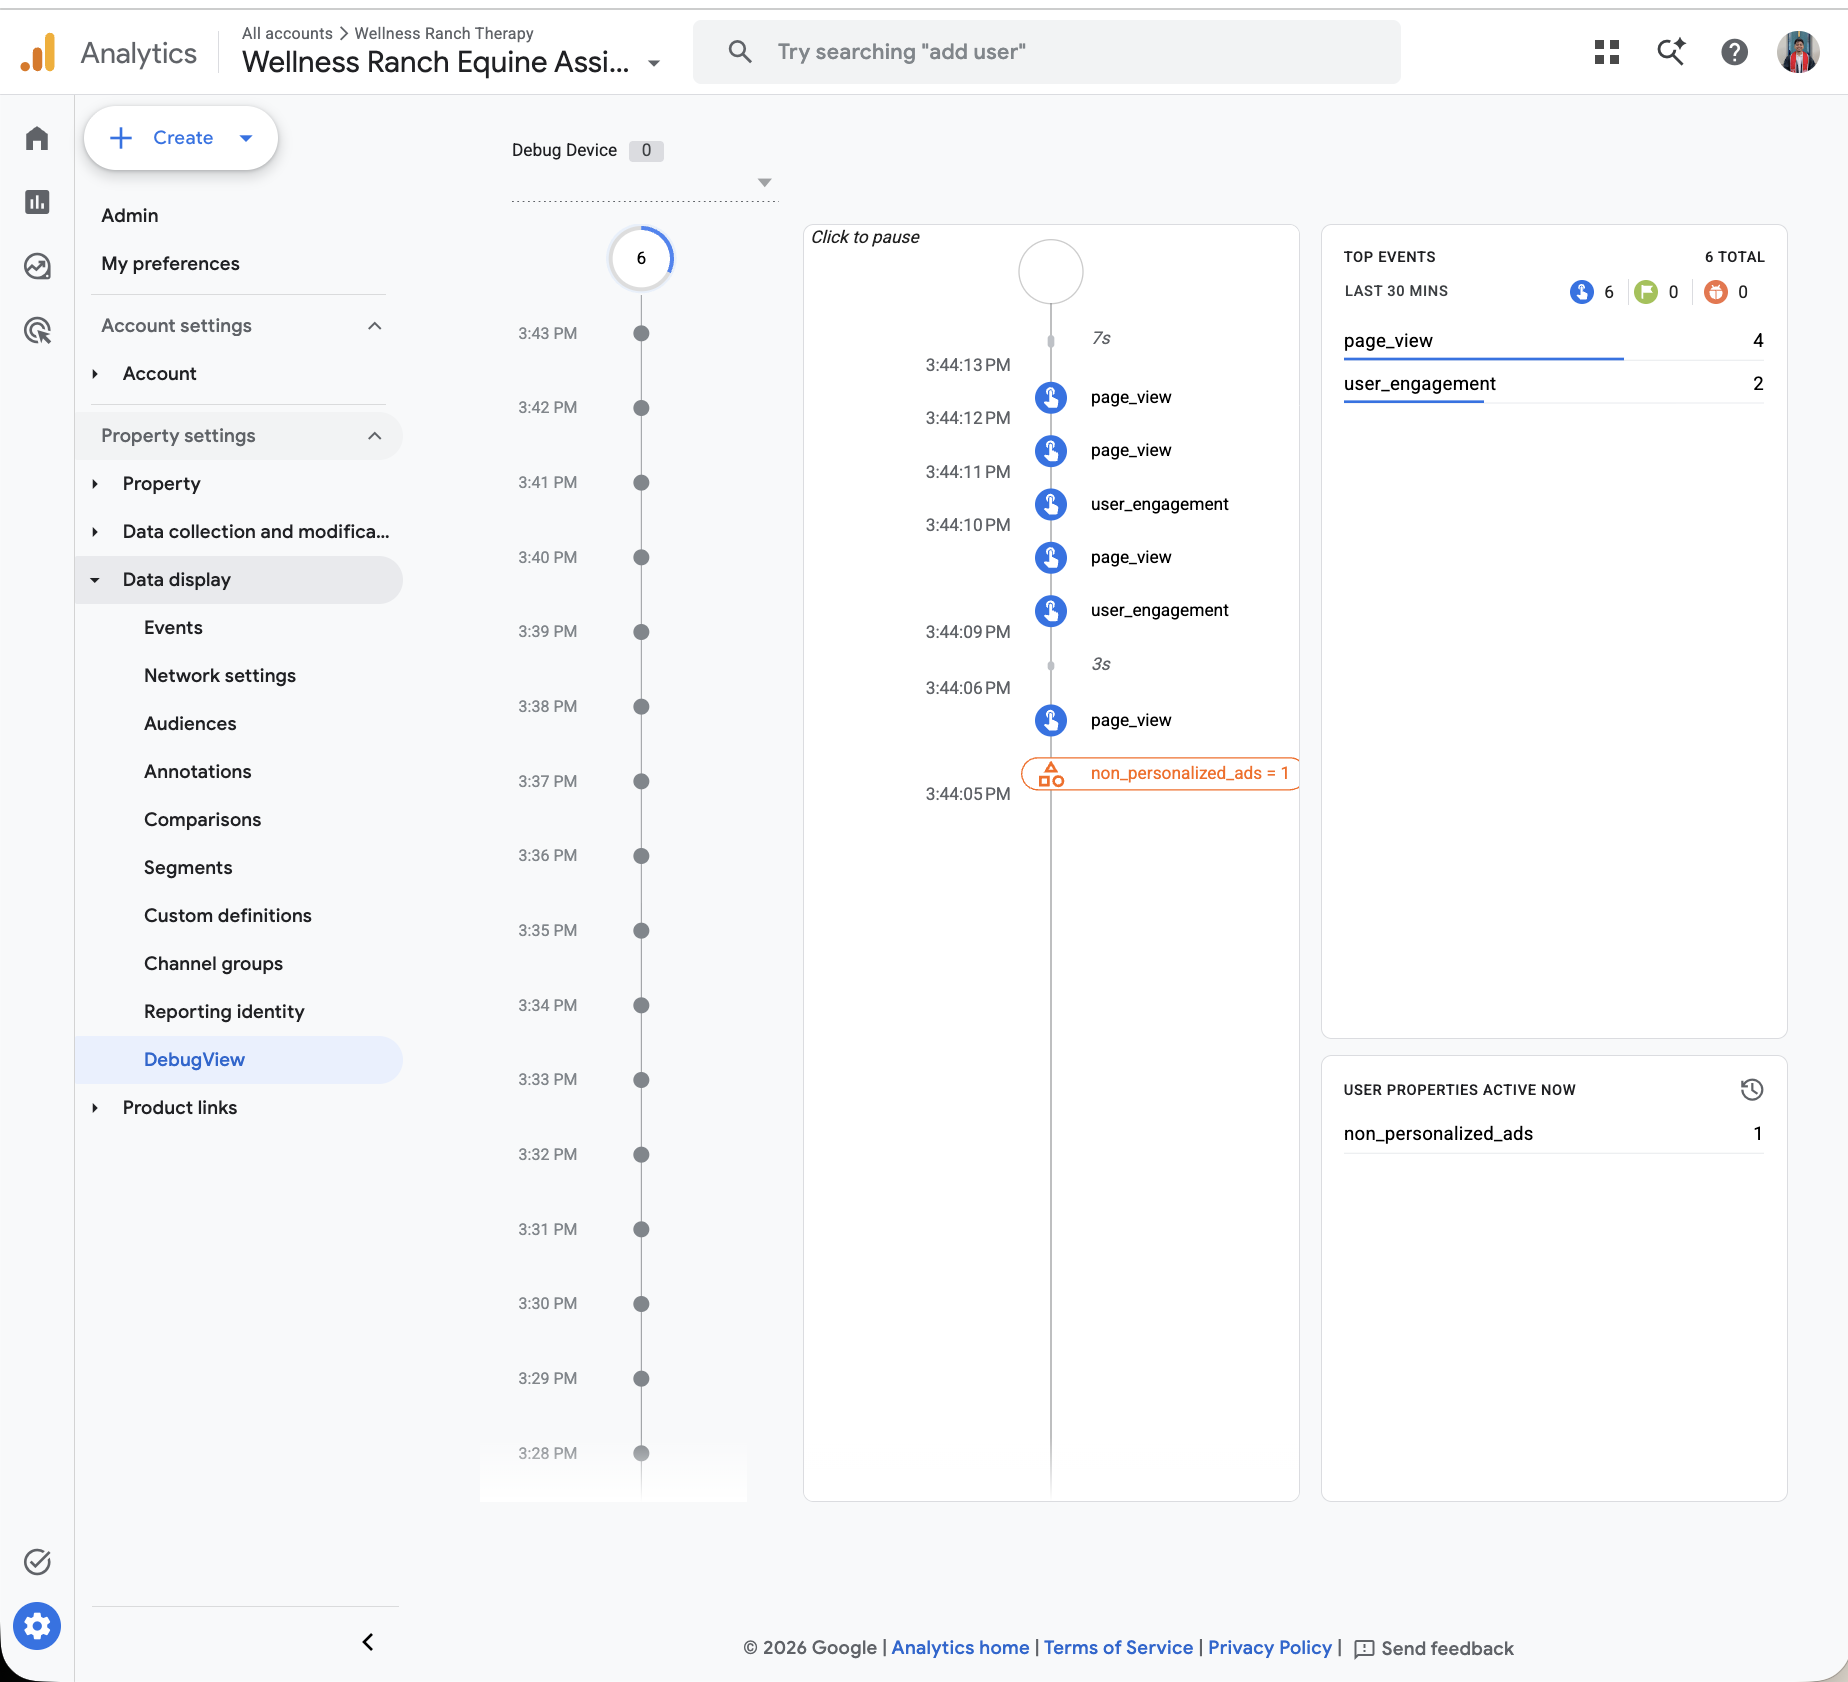
\includegraphics[width=1\linewidth,height=\textheight,keepaspectratio]{images/GA4_DebugView_Events.png}

}

\caption{GA4 DebugView event stream showing page\_view and
user\_engagement events}

\end{figure}%

Yes. Once we started browsing the site, events showed up in the
DebugView timeline within a few seconds (around 3:44 PM). Both
\texttt{page\_view} and \texttt{user\_engagement} fired like they're
supposed to, and the Top Events panel shows 6 total events in the last
30 minutes, which were 4 page views and 2 user engagement events. The
user property \texttt{non\_personalized\_ads} also came through, so GA4
is receiving user-level data along with events.

\subsubsection{Are the required parameters
there?}\label{are-the-required-parameters-there}

\begin{figure}[H]

{\centering 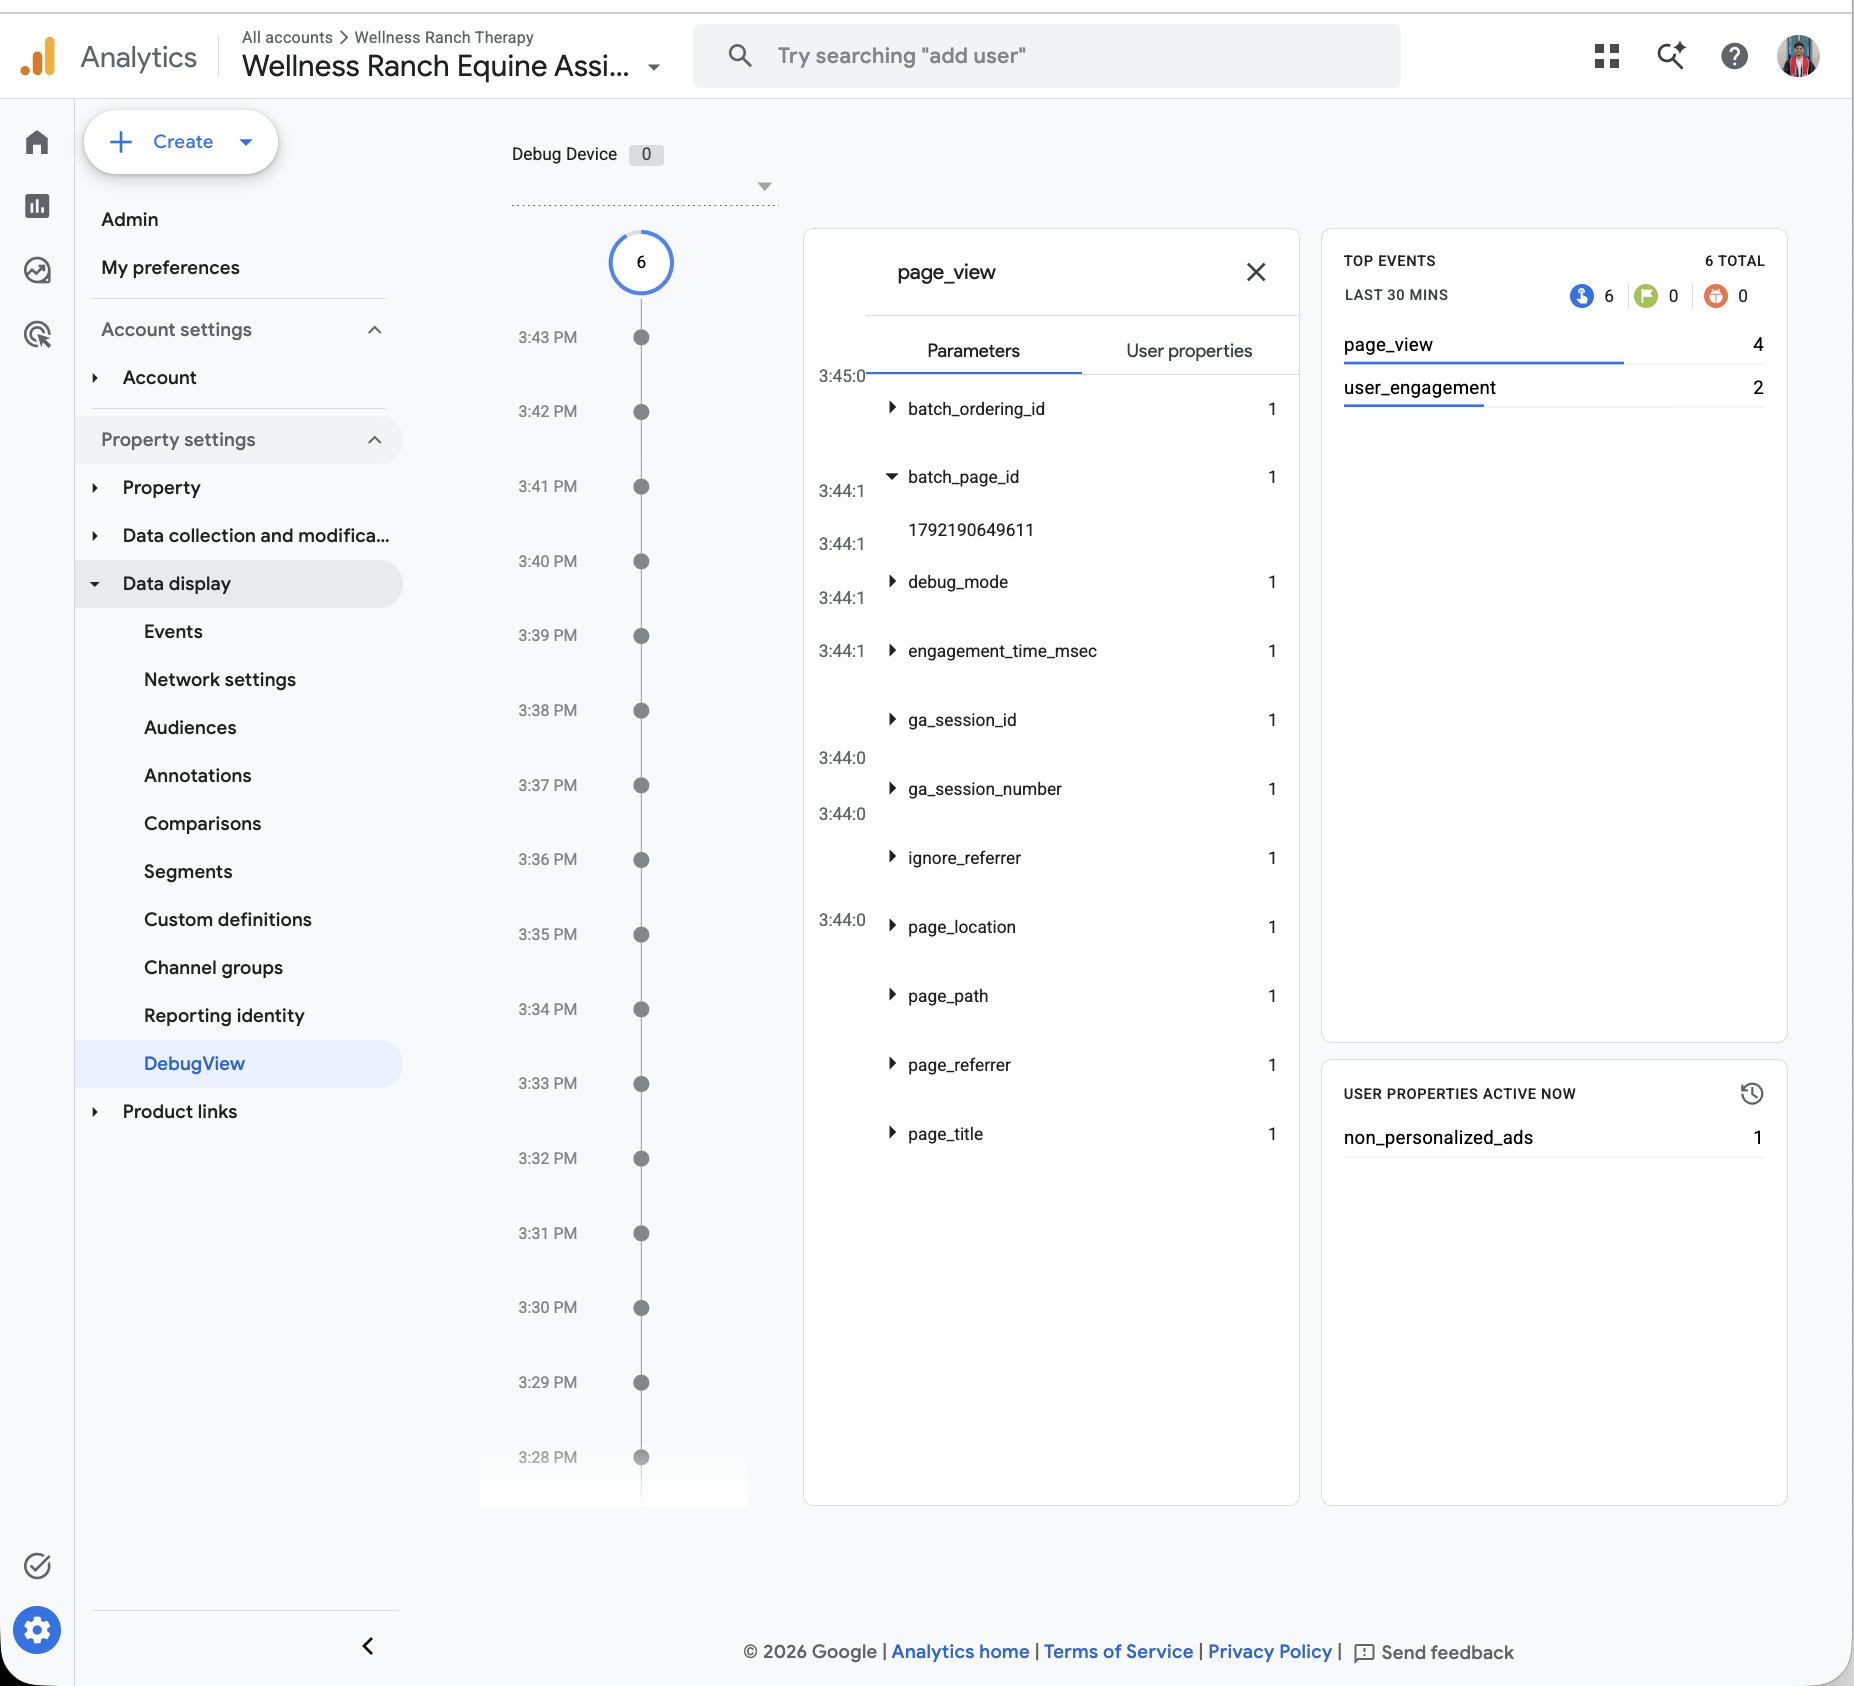
\includegraphics[width=1\linewidth,height=\textheight,keepaspectratio]{images/GA4_DebugView_BatchPageID.png}

}

\caption{page\_view event opened in DebugView showing its parameters}

\end{figure}%

Next we clicked into one of the \texttt{page\_view} events to see what
parameters came with it. All the main ones we need were there:

{\def\LTcaptype{none} % do not increment counter
\begin{longtable}[]{@{}ll@{}}
\toprule\noalign{}
Parameter & What it's for \\
\midrule\noalign{}
\endhead
\bottomrule\noalign{}
\endlastfoot
\texttt{page\_location} & the full URL of the page \\
\texttt{page\_path} & just the path part of the URL \\
\texttt{page\_title} & the name of the page \\
\texttt{page\_referrer} & where the user came from \\
\texttt{ga\_session\_id} & links the event to a session \\
\texttt{ga\_session\_number} & shows if it's a new or returning
session \\
\texttt{engagement\_time\_msec} & how long the user was engaged \\
\texttt{debug\_mode} & shows the hit came from our debug testing \\
\end{longtable}
}

There were also a couple of GA4 internal parameters like
\texttt{batch\_page\_id} (expanded in the screenshot, value
1792190649611\ldots) and \texttt{batch\_ordering\_id}. Each parameter
only showed up once per event, so nothing was missing or duplicated.

\subsubsection{Do the values make
sense?}\label{do-the-values-make-sense}

\begin{figure}[H]

{\centering 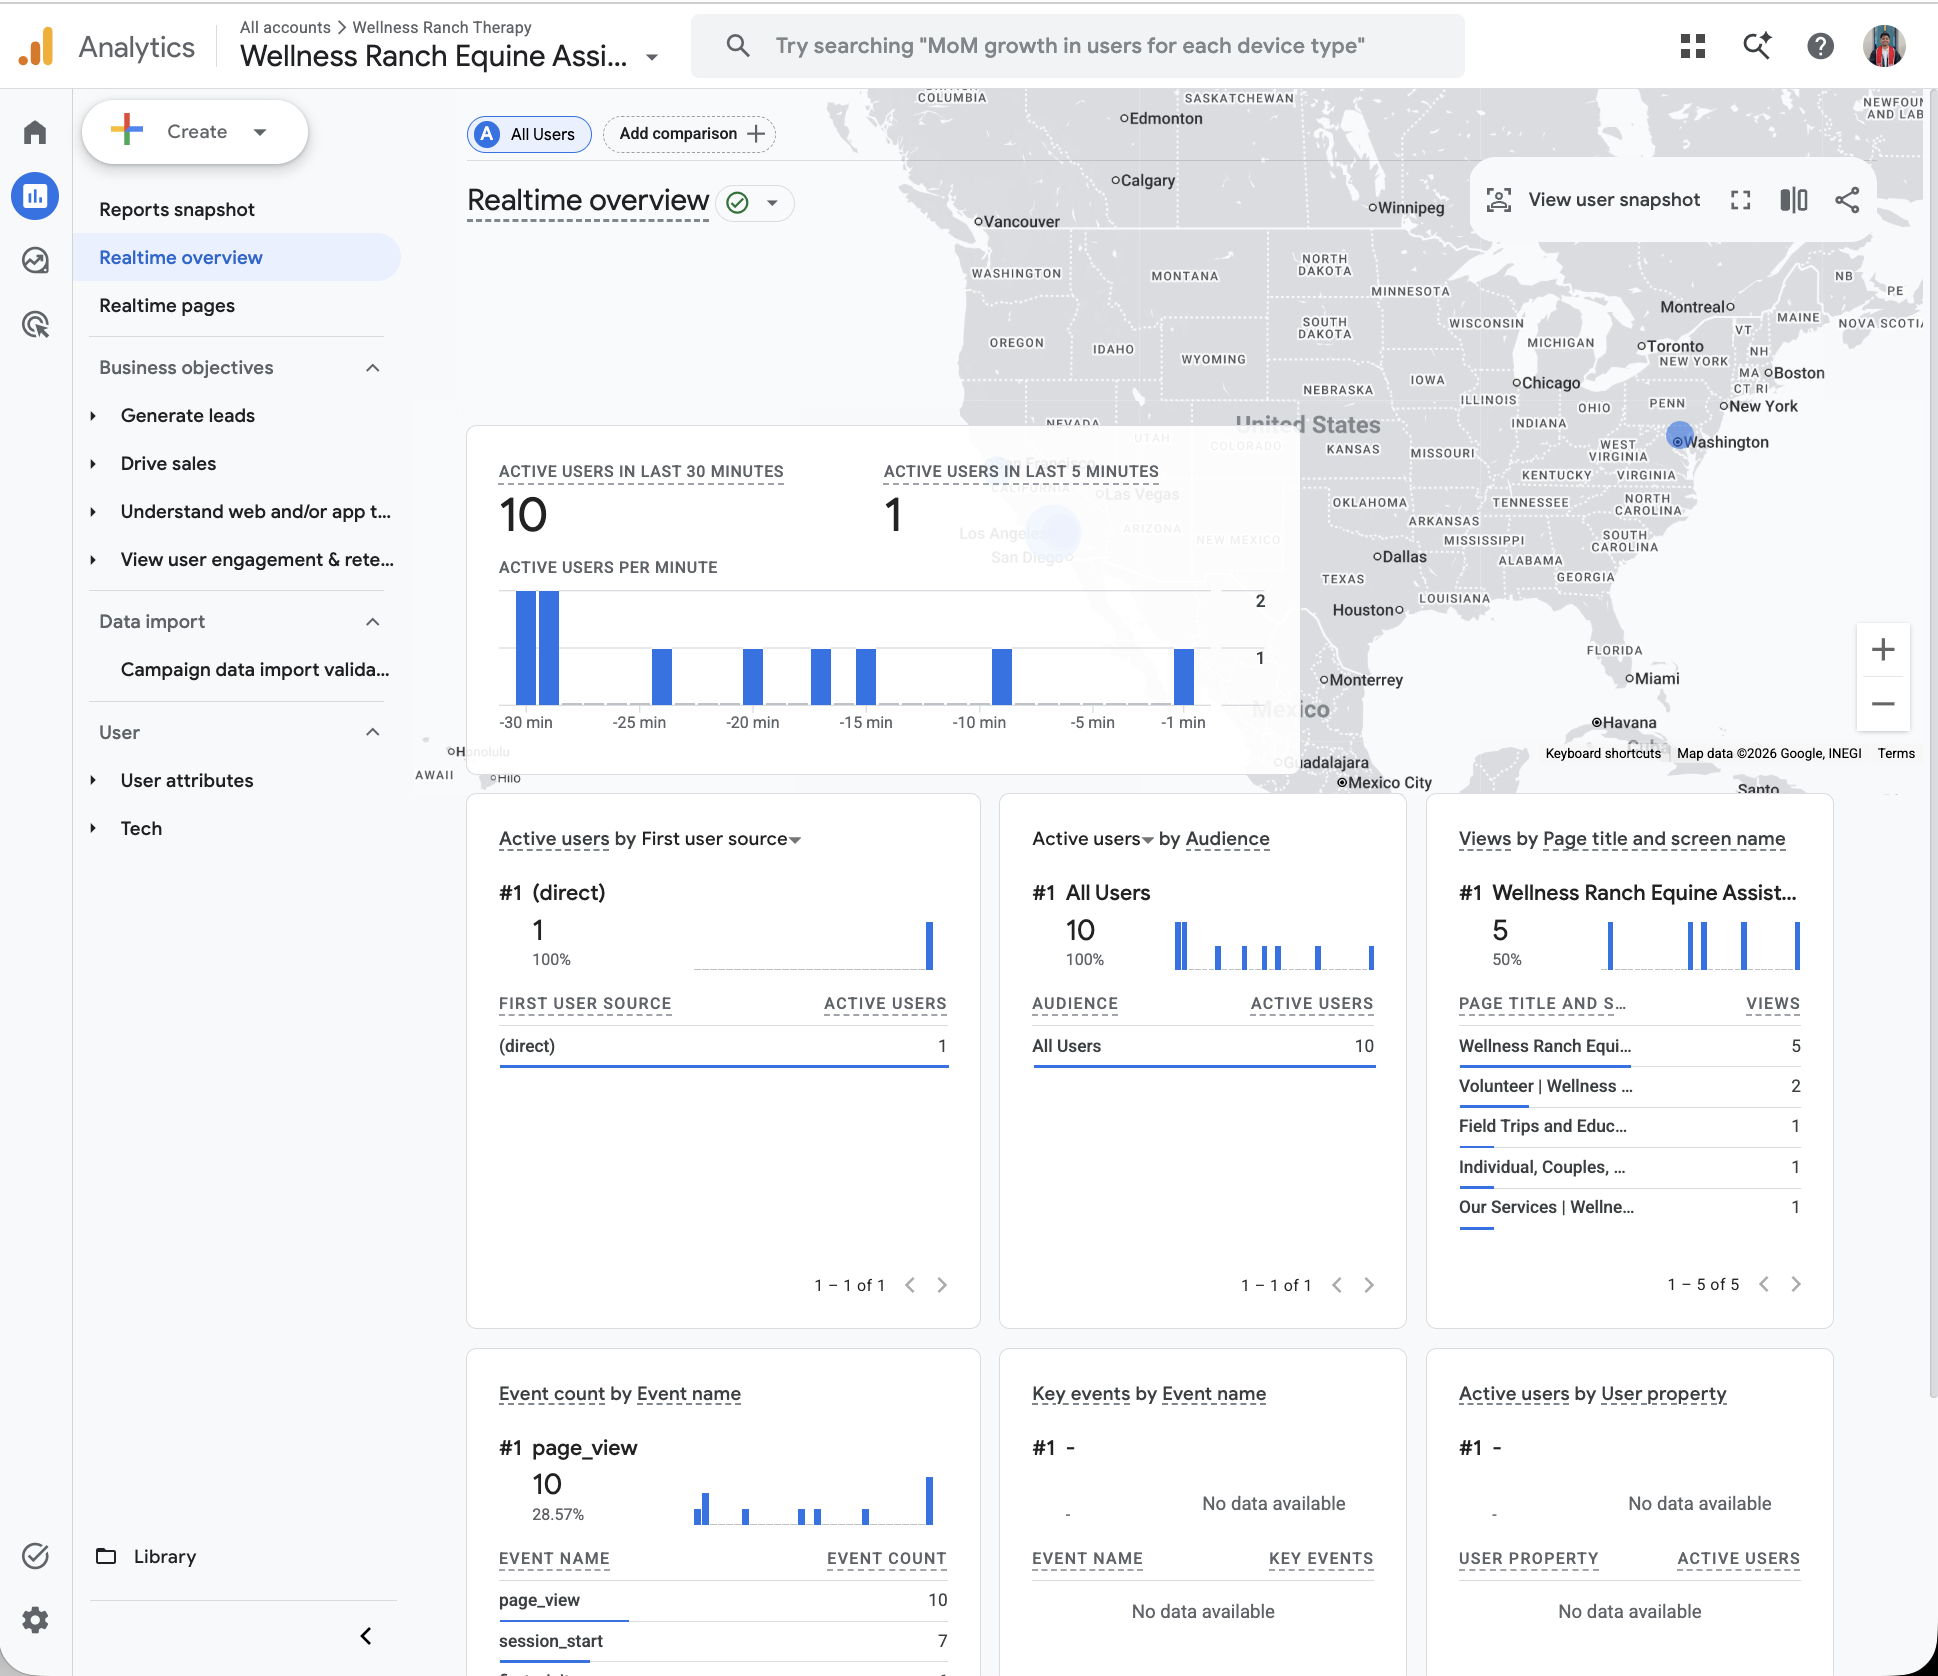
\includegraphics[width=1\linewidth,height=\textheight,keepaspectratio]{images/GA4_Realtime_PageView.png}

}

\caption{GA4 Realtime overview showing event counts and views by page
title}

\end{figure}%

To double check the values, we looked at the Realtime overview.
Everything lined up with how we tested the site:

\begin{itemize}
\tightlist
\item
  There were 10 active users in the last 30 minutes and 1 in the last 5
  minutes.
\item
  \texttt{page\_view} had 10 events and \texttt{session\_start} had 7.
  That makes sense since people usually view more than one page per
  session.
\item
  The page titles came through clean and match the real pages on the
  site: the homepage (\emph{Wellness Ranch Equine Assisted\ldots{}}) had
  the most views at 5, then \emph{Volunteer} (2), \emph{Field Trips and
  Education} (1), \emph{Individual, Couples\ldots{}} (1), and \emph{Our
  Services} (1).
\item
  The traffic source showed up as \texttt{(direct)}, which is right
  since we typed the URL in directly to test. This also shows why
  consistent UTMs matter later on (see Risks 5 and 9), because untagged
  traffic gets grouped as direct.
\end{itemize}

Since the page titles match the actual pages and follow the same format
every time, \texttt{page\_title} and \texttt{page\_location} are being
sent correctly across the site.

\subsubsection{Key event status}\label{key-event-status}

One thing we noticed is that the ``Key events by Event name'' card in
Realtime showed no data at the time of capture. This lines up with what
we found in the collection layer: \texttt{generate\_lead} was already
firing (see the Tag Assistant lead validation above), but it \textbf{had
not been marked as a key event yet}, so GA4 wasn't counting it as one.
We updated the key event configuration during testing, which is also why
we flagged key event changes as a risk (Risk 8).

\subsubsection{Summary}\label{summary}

{\def\LTcaptype{none} % do not increment counter
\begin{longtable}[]{@{}
  >{\raggedright\arraybackslash}p{(\linewidth - 4\tabcolsep) * \real{0.3333}}
  >{\raggedright\arraybackslash}p{(\linewidth - 4\tabcolsep) * \real{0.3333}}
  >{\raggedright\arraybackslash}p{(\linewidth - 4\tabcolsep) * \real{0.3333}}@{}}
\toprule\noalign{}
\begin{minipage}[b]{\linewidth}\raggedright
Check
\end{minipage} & \begin{minipage}[b]{\linewidth}\raggedright
Result
\end{minipage} & \begin{minipage}[b]{\linewidth}\raggedright
Status
\end{minipage} \\
\midrule\noalign{}
\endhead
\bottomrule\noalign{}
\endlastfoot
Events appear in DebugView & \texttt{page\_view},
\texttt{user\_engagement}, and \texttt{session\_start} received &
Pass \\
Required parameters populated & All page and session parameters present
on \texttt{page\_view} & Pass \\
Values sensible and consistent & Page titles and source match real site
pages and test behavior & Pass \\
Key events reporting & \texttt{generate\_lead} not yet marked as key
event at time of capture; updated during testing & Fixed during
testing \\
\end{longtable}
}

\subsection{Reporting Sanity Checks}\label{reporting-sanity-checks}

For this part, we checked that GA4's standard dimensions were filling in
correctly in the regular reports. We looked at four things: source /
medium, campaign, page title, and device category. For each one, we
checked whether the values made sense for Wellness Ranch and looked for
any \texttt{(not\ set)} values or numbers that didn't line up. All
reports use the same date range (last 28 days, Sep 18 -- Oct 15, 2026),
and the totals match across reports (902 sessions and 5,405 events), so
they're all looking at the same data.

One thing to know up front: in every report, the trend line is flat
until around October 7 and then jumps up. This suggests GA4 only started
collecting data around then, so even though the range says 28 days, it's
really about a week and a half of data. That also explains why almost
every user shows up as a new user (760 new out of 764 active users).

\subsubsection{Source / Medium}\label{source-medium}

\begin{figure}[H]

{\centering 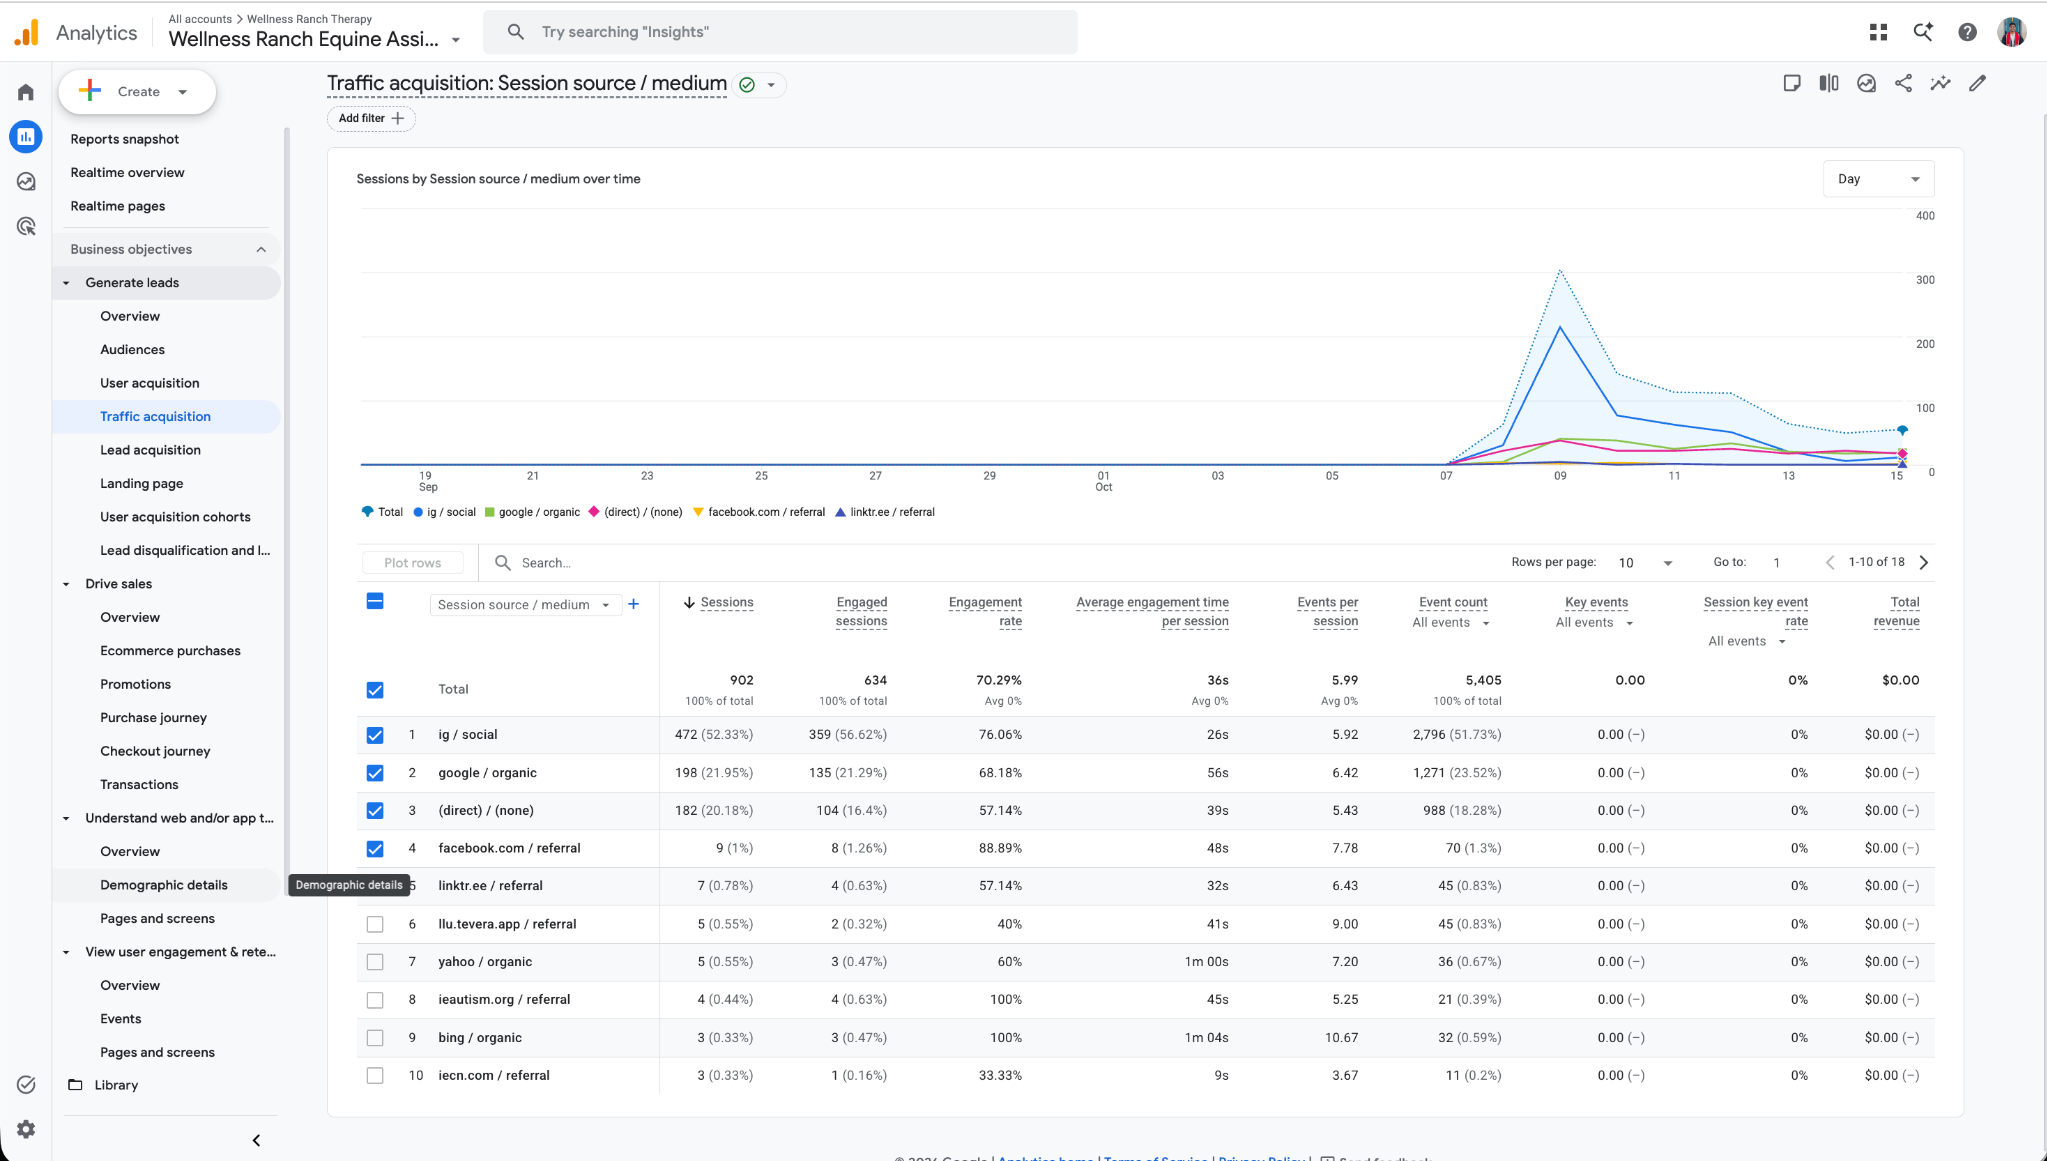
\includegraphics[width=1\linewidth,height=\textheight,keepaspectratio]{images/GA4_Source_Medium.png}

}

\caption{GA4 Traffic acquisition report by session source / medium}

\end{figure}%

Source / medium filled in correctly, with no \texttt{(not\ set)} values
in the top 10. The top sources were:

{\def\LTcaptype{none} % do not increment counter
\begin{longtable}[]{@{}lll@{}}
\toprule\noalign{}
Source / medium & Sessions & Share \\
\midrule\noalign{}
\endhead
\bottomrule\noalign{}
\endlastfoot
ig / social & 472 & 52.3\% \\
google / organic & 198 & 22.0\% \\
(direct) / (none) & 182 & 20.2\% \\
facebook.com / referral & 9 & 1.0\% \\
linktr.ee / referral & 7 & 0.8\% \\
\end{longtable}
}

These make sense for Wellness Ranch. Instagram is their biggest channel,
and \texttt{ig\ /\ social} is the tag Instagram adds automatically to
link-in-bio clicks, so it's being labeled correctly. Google organic
being second shows people are finding the site through search. The
smaller referral sources (like ieautism.org, iecn.com, and
llu.tevera.app) look like real community and partner sites, not spam,
which is a good sign.

\subsubsection{Campaign}\label{campaign}

\begin{figure}[H]

{\centering 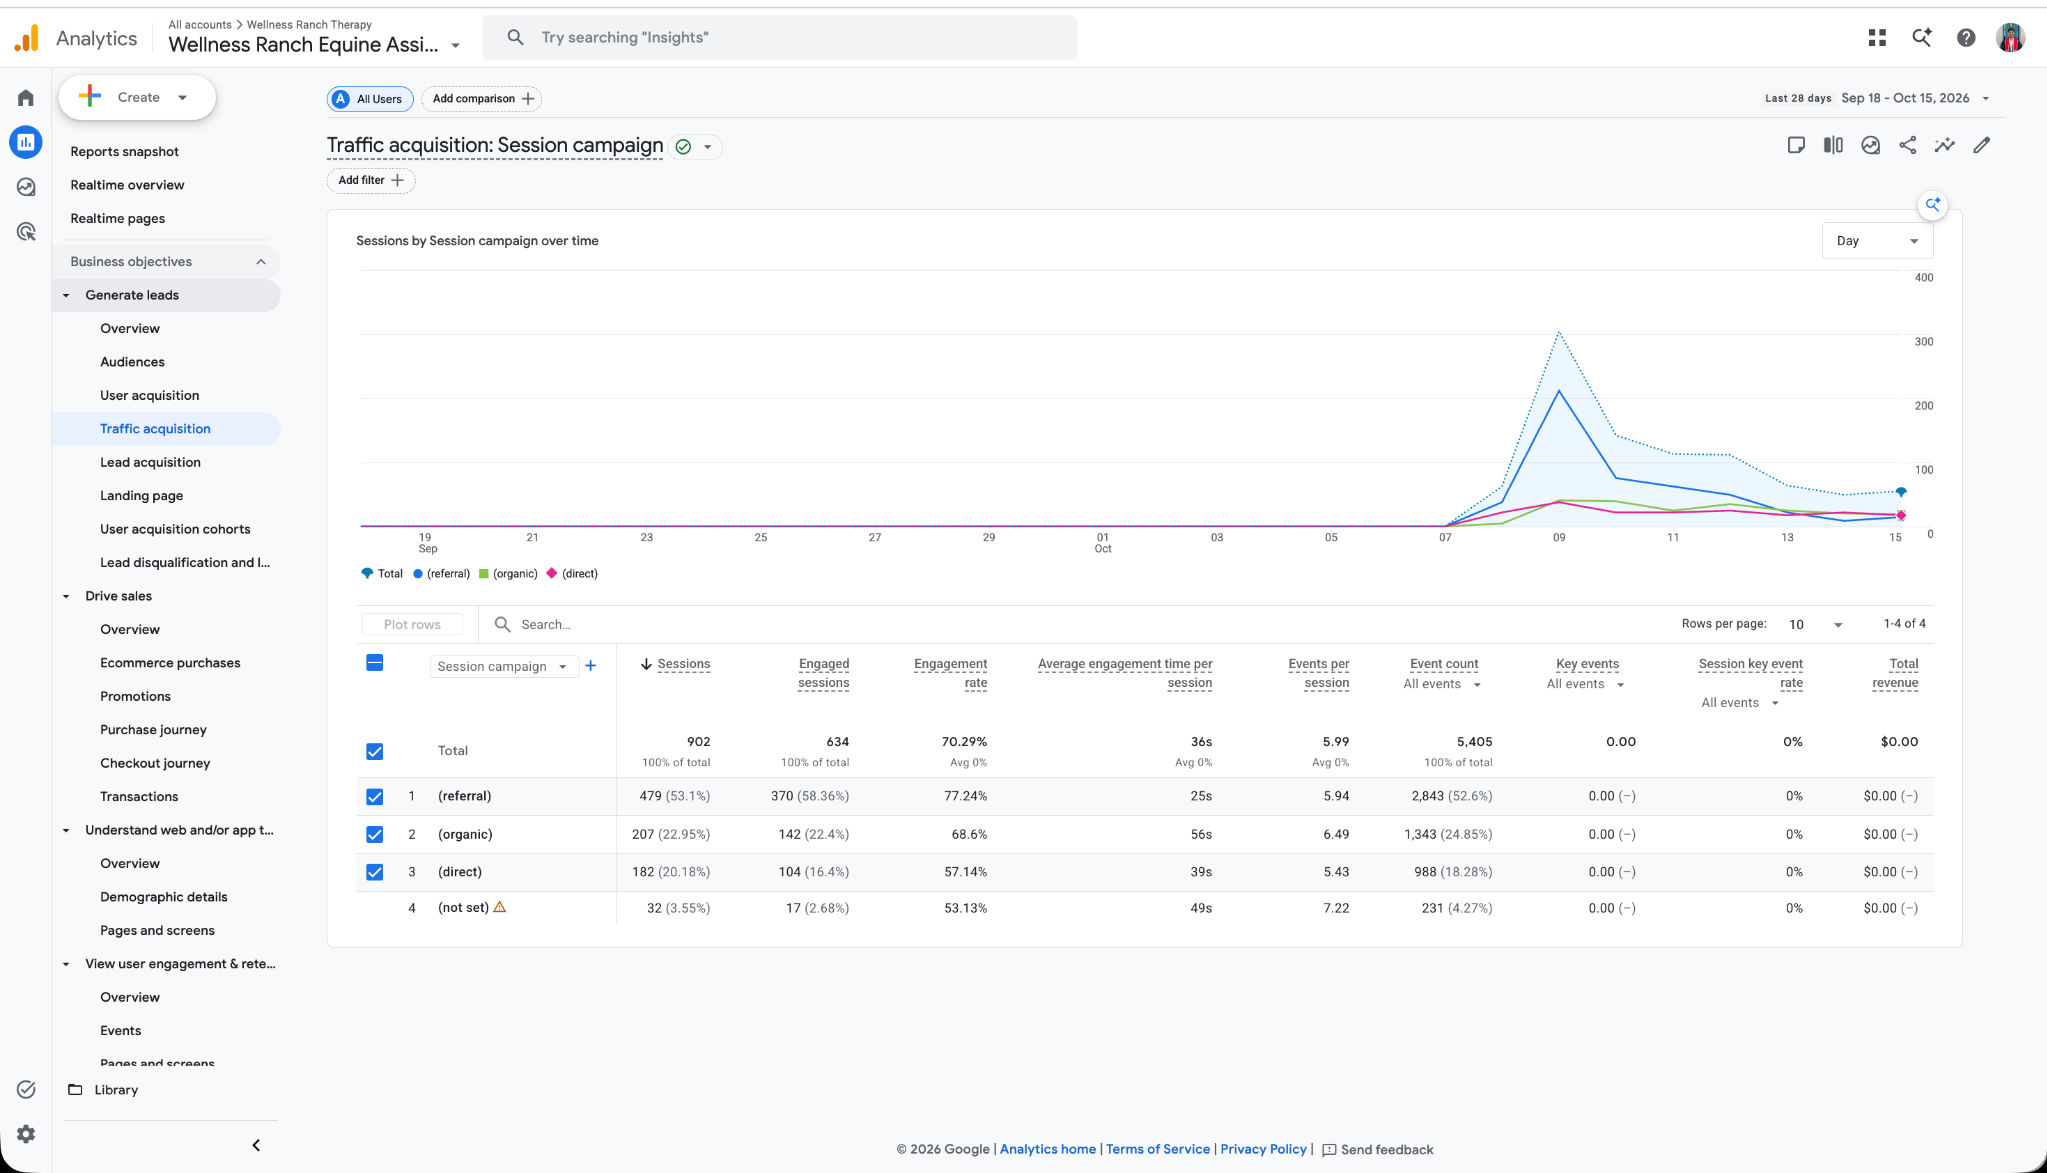
\includegraphics[width=1\linewidth,height=\textheight,keepaspectratio]{images/GA4_Campaign_Attribution.png}

}

\caption{GA4 Traffic acquisition report by session campaign}

\end{figure}%

Since Wellness Ranch isn't running any paid or named campaigns yet (the
Google Ad Grants account hasn't launched), we didn't expect to see real
campaign names. GA4 just used its default labels, which is normal:

{\def\LTcaptype{none} % do not increment counter
\begin{longtable}[]{@{}lll@{}}
\toprule\noalign{}
Session campaign & Sessions & Share \\
\midrule\noalign{}
\endhead
\bottomrule\noalign{}
\endlastfoot
(referral) & 479 & 53.1\% \\
(organic) & 207 & 23.0\% \\
(direct) & 182 & 20.2\% \\
(not set) & 32 & 3.6\% \\
\end{longtable}
}

The \texttt{(organic)} and \texttt{(direct)} numbers line up with the
source / medium report. Direct is exactly 182 in both, and organic (207)
matches Google + Yahoo + Bing organic plus a few smaller search engines
further down the list.

\textbf{Explaining the \texttt{(not\ set)}:} 32 sessions (3.6\%) came in
as \texttt{(not\ set)}. GA4 uses this when it can't figure out where a
session came from. Likely reasons are links that had a UTM source and
medium but no campaign name, or sessions that continued after a timeout
without a new page view to attach source info to. At 3.6\% it's small
and not a big concern, but it's another reason to set up a consistent
UTM naming standard before the Ad Grants campaigns go live (see Risks 5
and 9).

\subsubsection{Page Title}\label{page-title}

\begin{figure}[H]

{\centering 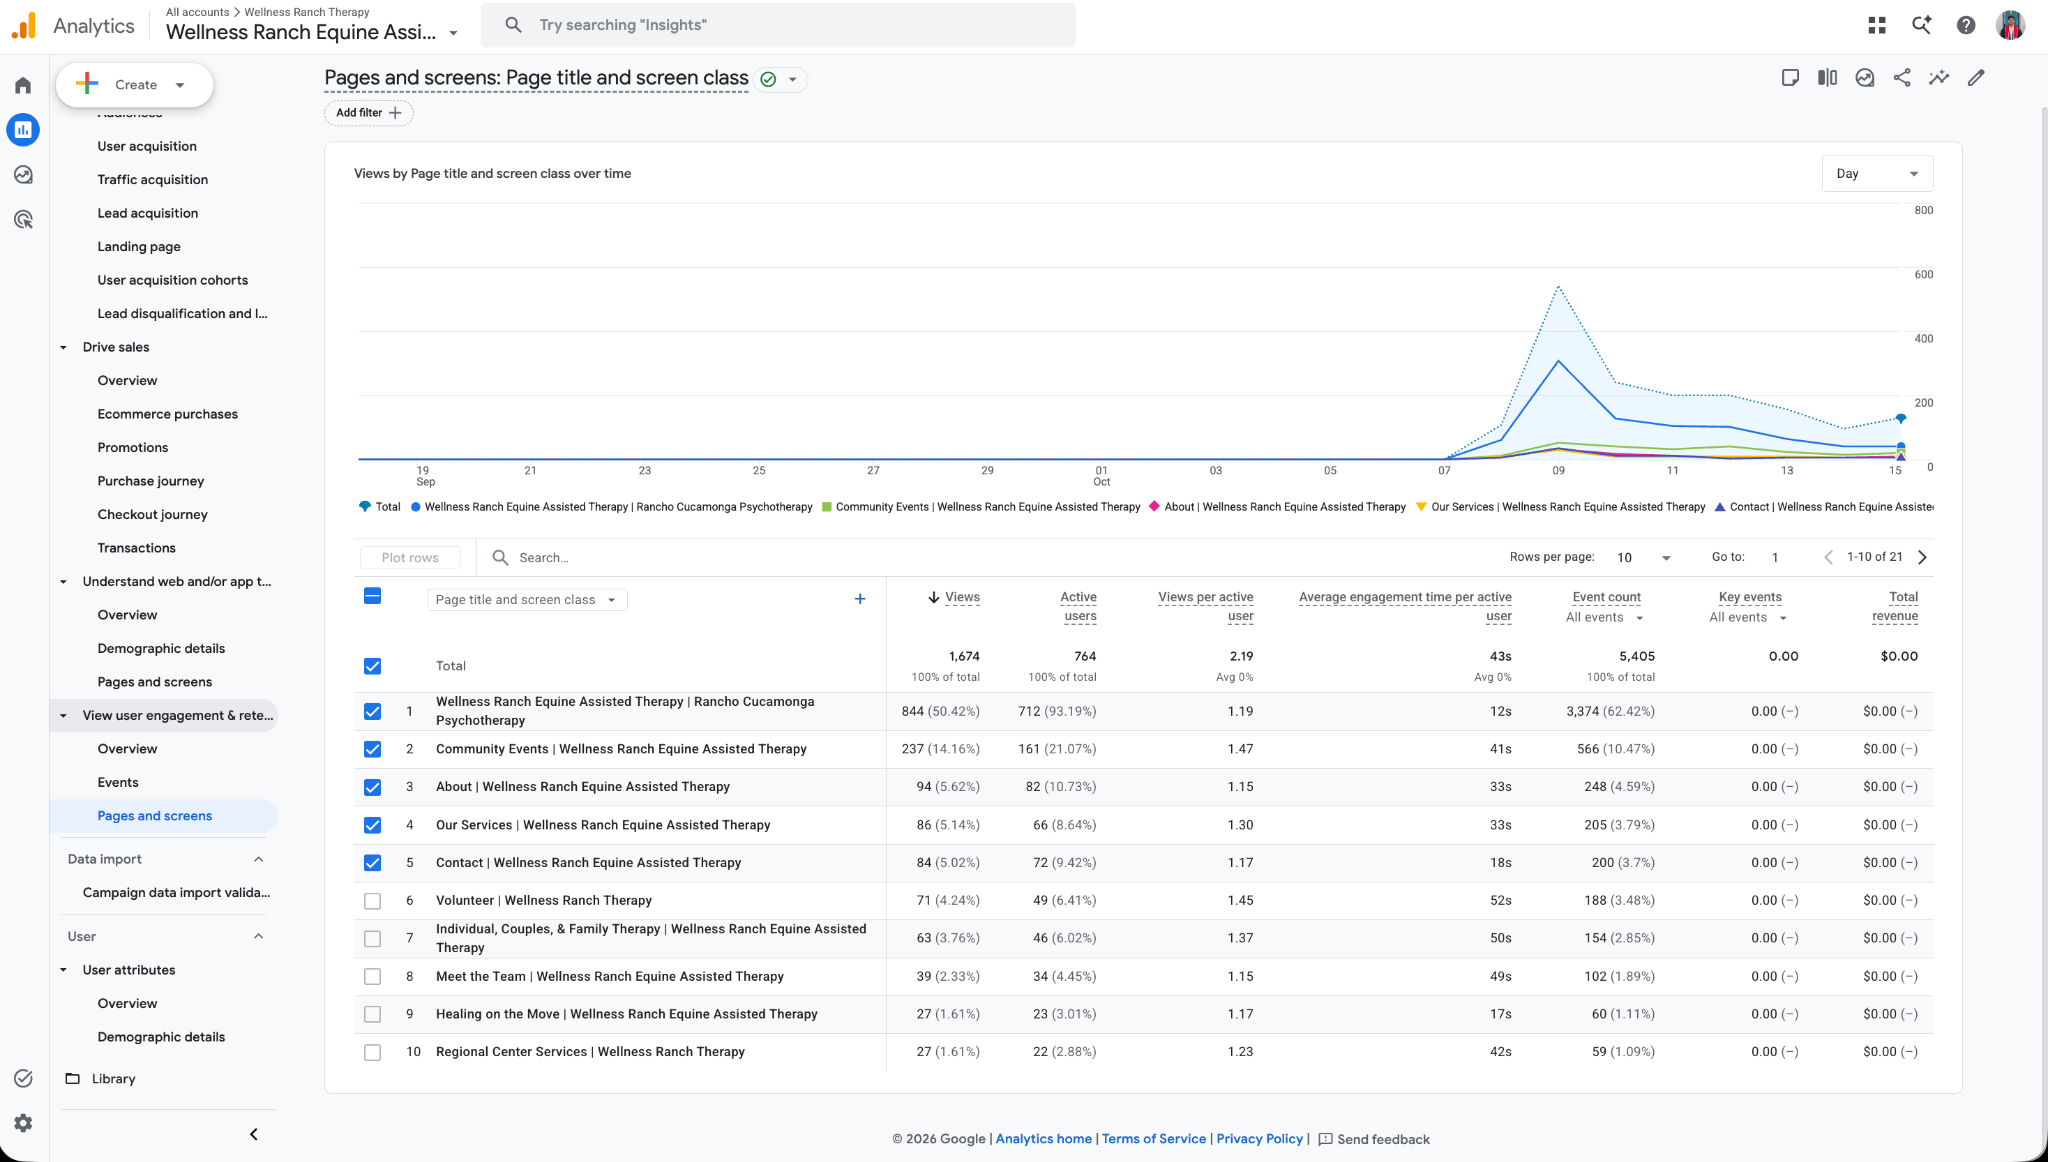
\includegraphics[width=1\linewidth,height=\textheight,keepaspectratio]{images/GA4_Page_Titles.png}

}

\caption{GA4 Pages and screens report by page title}

\end{figure}%

Page titles came through clean, with no \texttt{(not\ set)} values, and
they match the real pages on the site. There are 21 page titles total,
and the top ones were:

{\def\LTcaptype{none} % do not increment counter
\begin{longtable}[]{@{}
  >{\raggedright\arraybackslash}p{(\linewidth - 4\tabcolsep) * \real{0.3333}}
  >{\raggedright\arraybackslash}p{(\linewidth - 4\tabcolsep) * \real{0.3333}}
  >{\raggedright\arraybackslash}p{(\linewidth - 4\tabcolsep) * \real{0.3333}}@{}}
\toprule\noalign{}
\begin{minipage}[b]{\linewidth}\raggedright
Page title
\end{minipage} & \begin{minipage}[b]{\linewidth}\raggedright
Views
\end{minipage} & \begin{minipage}[b]{\linewidth}\raggedright
Share
\end{minipage} \\
\midrule\noalign{}
\endhead
\bottomrule\noalign{}
\endlastfoot
Wellness Ranch Equine Assisted Therapy \textbar{} Rancho Cucamonga
Psychotherapy (homepage) & 844 & 50.4\% \\
Community Events & 237 & 14.2\% \\
About & 94 & 5.6\% \\
Our Services & 86 & 5.1\% \\
Contact & 84 & 5.0\% \\
\end{longtable}
}

This makes sense, since the homepage is where most Instagram link-in-bio
traffic lands. Community Events being second is interesting, though, and
probably connects to event posts on Instagram.

\textbf{Small discrepancy:} The page titles aren't fully consistent.
Most end with ``\textbar{} Wellness Ranch \textbf{Equine Assisted}
Therapy,'' but a few (Volunteer and Regional Center Services) end with
``\textbar{} Wellness Ranch Therapy.'' This isn't a tracking error,
since GA4 is just reporting whatever title the page has. But it makes
reports a little messier, and it's something the Website \& SEO side
could clean up.

\textbf{Note on page location:} This report shows page titles, not full
URLs. We confirmed in the DebugView section that \texttt{page\_location}
is being sent with every \texttt{page\_view}, so the URL data is there,
it just isn't shown in this report.

\subsubsection{Device Category}\label{device-category}

\begin{figure}[H]

{\centering 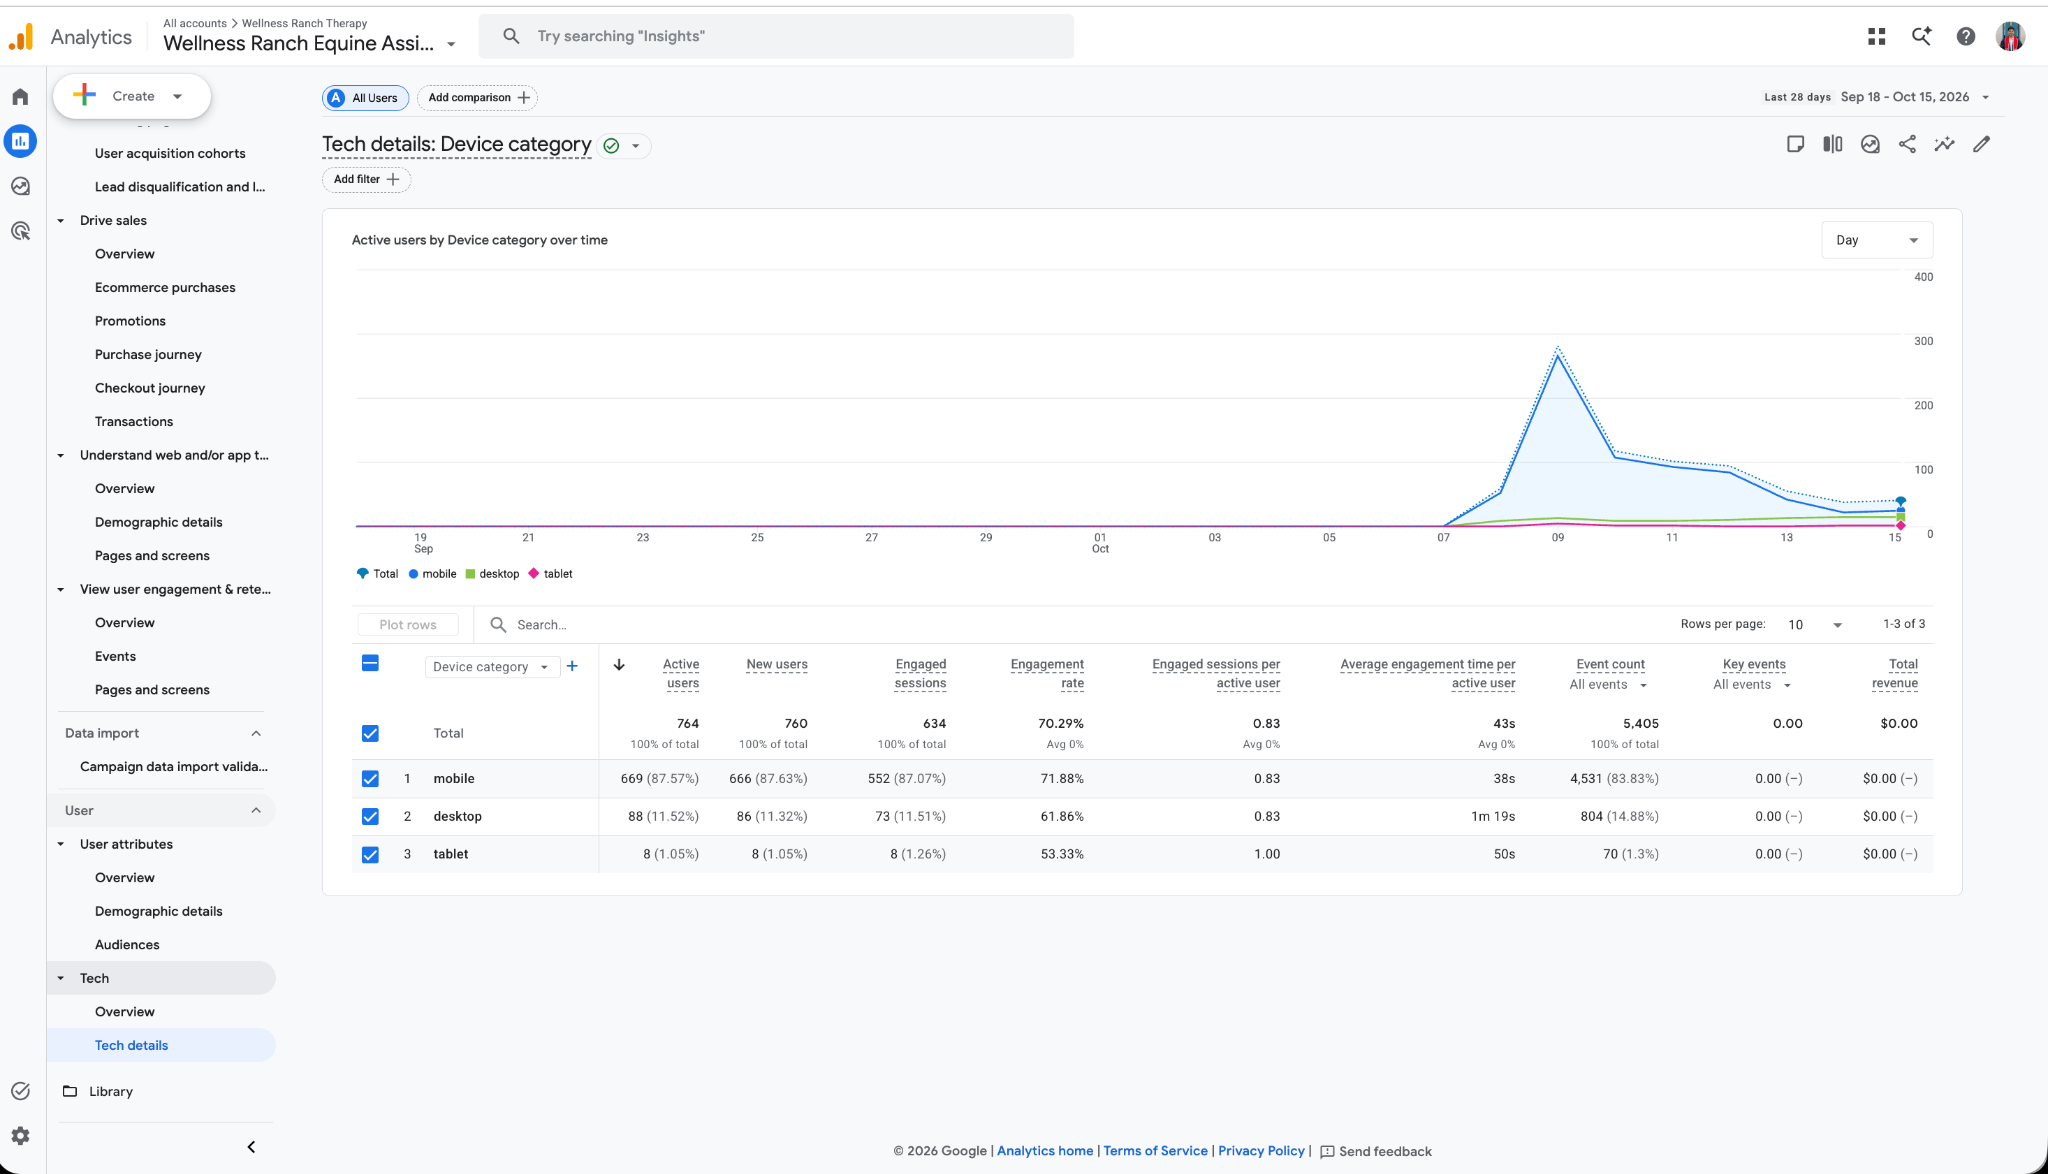
\includegraphics[width=1\linewidth,height=\textheight,keepaspectratio]{images/GA4_Device_Category.png}

}

\caption{GA4 Tech details report by device category}

\end{figure}%

Device category filled in correctly with no \texttt{(not\ set)} values:

{\def\LTcaptype{none} % do not increment counter
\begin{longtable}[]{@{}
  >{\raggedright\arraybackslash}p{(\linewidth - 8\tabcolsep) * \real{0.2000}}
  >{\raggedright\arraybackslash}p{(\linewidth - 8\tabcolsep) * \real{0.2000}}
  >{\raggedright\arraybackslash}p{(\linewidth - 8\tabcolsep) * \real{0.2000}}
  >{\raggedright\arraybackslash}p{(\linewidth - 8\tabcolsep) * \real{0.2000}}
  >{\raggedright\arraybackslash}p{(\linewidth - 8\tabcolsep) * \real{0.2000}}@{}}
\toprule\noalign{}
\begin{minipage}[b]{\linewidth}\raggedright
Device
\end{minipage} & \begin{minipage}[b]{\linewidth}\raggedright
Active users
\end{minipage} & \begin{minipage}[b]{\linewidth}\raggedright
Share
\end{minipage} & \begin{minipage}[b]{\linewidth}\raggedright
Engagement rate
\end{minipage} & \begin{minipage}[b]{\linewidth}\raggedright
Avg. engagement time
\end{minipage} \\
\midrule\noalign{}
\endhead
\bottomrule\noalign{}
\endlastfoot
mobile & 669 & 87.6\% & 71.9\% & 38s \\
desktop & 88 & 11.5\% & 61.9\% & 1m 19s \\
tablet & 8 & 1.1\% & 53.3\% & 50s \\
\end{longtable}
}

Mobile being almost 88\% of users lines up with Instagram being the top
traffic source, since most people click through from their phones.
Desktop users are a lot fewer but spend about twice as long on the site
(1m 19s vs 38s), which might mean desktop visitors are doing more
research.

\textbf{Small discrepancy:} The device rows add up to 765 users, but the
total says 764. That's normal in GA4, because if one person visits on
two different devices, they get counted once in each device row but only
once in the total.

\subsubsection{Summary}\label{summary-1}

{\def\LTcaptype{none} % do not increment counter
\begin{longtable}[]{@{}
  >{\raggedright\arraybackslash}p{(\linewidth - 6\tabcolsep) * \real{0.2500}}
  >{\raggedright\arraybackslash}p{(\linewidth - 6\tabcolsep) * \real{0.2500}}
  >{\raggedright\arraybackslash}p{(\linewidth - 6\tabcolsep) * \real{0.2500}}
  >{\raggedright\arraybackslash}p{(\linewidth - 6\tabcolsep) * \real{0.2500}}@{}}
\toprule\noalign{}
\begin{minipage}[b]{\linewidth}\raggedright
Dimension
\end{minipage} & \begin{minipage}[b]{\linewidth}\raggedright
Populated correctly?
\end{minipage} & \begin{minipage}[b]{\linewidth}\raggedright
(not set) / discrepancies
\end{minipage} & \begin{minipage}[b]{\linewidth}\raggedright
Status
\end{minipage} \\
\midrule\noalign{}
\endhead
\bottomrule\noalign{}
\endlastfoot
Source / medium & Yes, values match real channels & None in top 10 &
Pass \\
Campaign & Yes, default labels as expected (no campaigns running yet) &
32 sessions (3.6\%) \texttt{(not\ set)}, likely missing UTM campaign or
timed-out sessions & Pass (needs UTM standard) \\
Page title & Yes, matches real site pages & Inconsistent title suffixes
on some pages & Pass \\
Page location & Confirmed in DebugView & Not shown in this report &
Pass \\
Device category & Yes & Device rows sum to 765 vs 764 total (users on
multiple devices) & Pass \\
\end{longtable}
}

Also worth noting: \textbf{Key events show 0 in every report.} This
matches what we found earlier, where \texttt{generate\_lead} was firing
but hadn't been marked as a key event yet during this date range.

\subsection{BigQuery Export
Validation}\label{bigquery-export-validation}

BigQuery export sends GA4's raw, event-level data into a BigQuery
dataset, where it can be queried directly with SQL. This matters because
the standard GA4 reports are aggregated and can be sampled or
thresholded, while the export gives access to every event and parameter.
For this project, it would let the team check \texttt{generate\_lead}
events individually and build attribution analysis that can be
reproduced later.

\subsubsection{Export Status}\label{export-status}

According to the team's review of the GA4 property, there is no active
BigQuery export connection. This would be confirmed under Admin →
Product links → BigQuery links. A screenshot of this page was not
captured during testing.

Because the export is not set up, we were not able to complete the
following checks:

\begin{itemize}
\tightlist
\item
  Confirm that daily \texttt{events\_YYYYMMDD} tables are being created
\item
  Compare event counts in BigQuery to the GA4 interface
\item
  Confirm that \texttt{generate\_lead} parameters can be pulled out at
  the event level
\item
  Check for duplicate lead events using raw timestamps and session IDs
\end{itemize}

\subsubsection{Planned Validation Once Export Is
Enabled}\label{planned-validation-once-export-is-enabled}

If the team gets the required permissions and turns on the export, these
are the checks we would run:

{\def\LTcaptype{none} % do not increment counter
\begin{longtable}[]{@{}
  >{\raggedright\arraybackslash}p{(\linewidth - 4\tabcolsep) * \real{0.3333}}
  >{\raggedright\arraybackslash}p{(\linewidth - 4\tabcolsep) * \real{0.3333}}
  >{\raggedright\arraybackslash}p{(\linewidth - 4\tabcolsep) * \real{0.3333}}@{}}
\toprule\noalign{}
\begin{minipage}[b]{\linewidth}\raggedright
Check
\end{minipage} & \begin{minipage}[b]{\linewidth}\raggedright
How we would test it
\end{minipage} & \begin{minipage}[b]{\linewidth}\raggedright
What would count as a pass
\end{minipage} \\
\midrule\noalign{}
\endhead
\bottomrule\noalign{}
\endlastfoot
Daily tables created & Look for \texttt{events\_} tables in the
\texttt{analytics\_\textless{}property\_id\textgreater{}} dataset & A
new table appears each day \\
Event counts match & Compare daily \texttt{page\_view} and
\texttt{generate\_lead} counts to GA4 reports & Counts are close (small
differences are normal) \\
Lead parameters present & Query \texttt{event\_params} on
\texttt{generate\_lead} events & Expected parameters are populated \\
Duplicate leads & Look for multiple \texttt{generate\_lead} events in
the same session within a few seconds & One lead event per submission \\
\end{longtable}
}

A simple starting query for the count comparison would look like this:

``\texttt{sql\ SELECT\ \ \ event\_date,\ \ \ event\_name,\ \ \ COUNT(*)\ AS\ event\_count\ FROM}project\_id.analytics\_property\_id.events\_*`
WHERE event\_name IN

\section{Issues Log: Findings and Fixes
Attempted}\label{issues-log-findings-and-fixes-attempted}

\subsection{Issues Identified}\label{issues-identified}

The table below pulls together the issues found across the collection
layer, DebugView, reporting, and BigQuery checks.

{\def\LTcaptype{none} % do not increment counter
\begin{longtable}[]{@{}
  >{\raggedright\arraybackslash}p{(\linewidth - 8\tabcolsep) * \real{0.2000}}
  >{\raggedright\arraybackslash}p{(\linewidth - 8\tabcolsep) * \real{0.2000}}
  >{\raggedright\arraybackslash}p{(\linewidth - 8\tabcolsep) * \real{0.2000}}
  >{\raggedright\arraybackslash}p{(\linewidth - 8\tabcolsep) * \real{0.2000}}
  >{\raggedright\arraybackslash}p{(\linewidth - 8\tabcolsep) * \real{0.2000}}@{}}
\toprule\noalign{}
\begin{minipage}[b]{\linewidth}\raggedright
\#
\end{minipage} & \begin{minipage}[b]{\linewidth}\raggedright
Issue
\end{minipage} & \begin{minipage}[b]{\linewidth}\raggedright
Where it was found
\end{minipage} & \begin{minipage}[b]{\linewidth}\raggedright
Severity
\end{minipage} & \begin{minipage}[b]{\linewidth}\raggedright
Status
\end{minipage} \\
\midrule\noalign{}
\endhead
\bottomrule\noalign{}
\endlastfoot
1 & \texttt{generate\_lead} was firing but was not marked as a key event
& Realtime and standard reports (key events showed 0) & High & Fixed
during testing \\
2 & Duplicate lead testing was limited to one submission & Tag Assistant
& Medium & Open \\
3 & 32 sessions (3.6\%) had a \texttt{(not\ set)} campaign & Campaign
report & Low & Open \\
4 & Page title suffixes are inconsistent across pages & Pages and
screens report & Low & Open \\
5 & BigQuery export is not active & GA4 BigQuery links & High & Open \\
6 & Data collection appears to have started around October 7, so the
28-day range only has about a week and a half of data & All standard
reports & Medium & Limitation \\
\end{longtable}
}

\subsection{Fixes Attempted and Current
Status}\label{fixes-attempted-and-current-status}

\textbf{Issue 1: Key event configuration.} This was the only issue fixed
during testing. We marked \texttt{generate\_lead} as a key event in GA4
on October 16, 2026. GA4 does not apply key event changes to past data,
so conversions will only start showing up in reports from that date
forward. That is why key events still show 0 for the Sep 18 to Oct 15
range. Any future reporting should note the October 16 change date (see
Risk 8).

\textbf{Issue 2: Duplicate lead testing.} No fix needed yet, since the
one test submission produced one event. More tests across desktop and
mobile, including double clicks and page refreshes, are needed before we
can rule out duplicates (see Risk 1).

\textbf{Issue 3: \texttt{(not\ set)} campaign values.} No fix attempted.
At 3.6\% it is small, but it should be addressed with a UTM naming
standard before the Google Ad Grants campaigns launch (see Risk 5).

\textbf{Issue 4: Inconsistent page titles.} This is a website issue, not
a tracking error. We are passing it to the Website \& SEO side to
standardize the title suffixes.

\textbf{Issue 5: BigQuery export.} No fix attempted, since enabling the
export requires permissions on a Google Cloud project. The next step is
to confirm who owns the GA4 property and request access (see Risk 7).

\textbf{Issue 6: Short data window.} This cannot be fixed after the
fact. Future reports should use date ranges that start on or after
October 7 so the numbers are not misread as a full month. Although the
QA testing confirmed that the Google tag, page views, form interactions,
and \texttt{generate\_lead} events are being received by GA4, several
risks could affect data quality over time. These risks should be
monitored as the Wellness Ranch website, campaigns, and tracking
configuration change.

\subsection{Risk 1: Duplicate Lead
Events}\label{risk-1-duplicate-lead-events}

\textbf{Risk description:} A single contact-form submission could
generate more than one \texttt{generate\_lead} event because of repeated
clicks, page refreshes, confirmation-page reloads, or overlapping tags.

\textbf{Why it matters:} Duplicate lead events would inflate the number
of conversions and make conversion rates, campaign comparisons, and
lead-generation reports inaccurate.

\textbf{Likely impact:} Medium

\textbf{Mitigation strategy:} Test multiple form submissions across
desktop and mobile devices. Use a unique submission or
confirmation-state trigger, prevent repeated event firing, and compare
form-submission records with GA4 event counts. Review unusual spikes in
\texttt{generate\_lead} events.

\subsection{Risk 2: Embedded or Third-Party Form Tracking
Limitations}\label{risk-2-embedded-or-third-party-form-tracking-limitations}

\textbf{Risk description:} If the contact form is embedded from a
third-party provider, GA4 or Google Tag Manager may not consistently
detect form starts, successful submissions, or confirmation states.

\textbf{Why it matters:} Missing or incomplete form events could
undercount meaningful conversions and make the website appear less
effective than it actually is.

\textbf{Likely impact:} High

\textbf{Mitigation strategy:} Confirm whether the form is hosted on the
Wellness Ranch website or an external platform. Test successful
submissions, validation errors, abandoned forms, and confirmation
messages. If necessary, use a reliable data-layer event, thank-you-page
trigger, or server-side confirmation from the form provider.

\subsection{Risk 3: Consent Settings May Suppress
Events}\label{risk-3-consent-settings-may-suppress-events}

\textbf{Risk description:} Consent choices, browser privacy settings, or
ad blockers may prevent some users and events from being recorded.

\textbf{Why it matters:} GA4 reports may undercount users, sessions,
engagement, and conversions. Suppression may also vary by device,
browser, or audience segment, which can create biased comparisons.

\textbf{Likely impact:} Medium

\textbf{Mitigation strategy:} Test tracking with analytics consent
accepted and declined. Document which events are expected to be blocked
under each consent state. Interpret trends as observed activity rather
than a complete count of all website activity, and monitor consent rates
over time.

\subsection{Risk 4: Cross-Domain Tracking
Limitations}\label{risk-4-cross-domain-tracking-limitations}

\textbf{Risk description:} If users move from the Wellness Ranch website
to an external form, scheduling system, donation platform, or payment
page, the user journey may not remain connected across domains.

\textbf{Why it matters:} Conversions may be attributed to direct traffic
or a referral instead of the original campaign, keyword, or landing
page. This could weaken attribution analysis and distort campaign
performance.

\textbf{Likely impact:} High

\textbf{Mitigation strategy:} Identify all external domains used in the
user journey. Configure cross-domain measurement when supported, exclude
trusted domains from unwanted-referral lists, and test the complete path
from advertisement or landing page through the final conversion. If
cross-domain tracking is not possible, report external conversions
separately and document the limitation.

\subsection{Risk 5: Incomplete or Inconsistent UTM
Parameters}\label{risk-5-incomplete-or-inconsistent-utm-parameters}

\textbf{Risk description:} Campaign links may be created without UTMs or
may use inconsistent capitalization, abbreviations, or naming
conventions.

\textbf{Why it matters:} Traffic may be grouped into
\texttt{(not\ set)}, direct traffic, or inconsistent campaign
categories. This makes it difficult to compare channels, campaigns,
advertisements, and keyword-intent groups.

\textbf{Likely impact:} Medium

\textbf{Mitigation strategy:} Create a shared UTM naming standard for
source, medium, campaign, content, and term. Use a campaign URL builder
or tracking template, review links before launch, and periodically audit
GA4 acquisition reports for missing or inconsistent values.

\subsection{Risk 6: Low Traffic and Conversion
Volume}\label{risk-6-low-traffic-and-conversion-volume}

\textbf{Risk description:} Wellness Ranch may receive a limited number
of website visitors, advertisement clicks, and conversions during the
measurement period.

\textbf{Why it matters:} Small sample sizes can cause large percentage
changes from only a few users. Low volume also makes it difficult to
determine whether differences between campaigns or keyword groups are
meaningful.

\textbf{Likely impact:} Medium

\textbf{Mitigation strategy:} Report counts together with rates and
avoid drawing strong conclusions from very small groups. Use longer
observation periods, combine closely related categories when
appropriate, and clearly label results as directional when sample sizes
are limited.

\subsection{Risk 7: BigQuery Export Is Not Currently
Active}\label{risk-7-bigquery-export-is-not-currently-active}

\textbf{Risk description:} The GA4 property does not currently have an
active BigQuery export connection.

\textbf{Why it matters:} Without BigQuery, the team cannot independently
query raw event-level data, extract parameters at scale, or build
reproducible attribution analyses from the exported event data.

\textbf{Likely impact:} High

\textbf{Mitigation strategy:} Confirm whether BigQuery export is
available and obtain the required project permissions. If export cannot
be enabled, document GA4 as the primary source, preserve regular report
exports, and maintain a consistent data dictionary for events and
parameters. Avoid presenting GA4 interface totals as equivalent to a
complete raw-data export.

\subsection{Risk 8: Changes to Key Event
Configuration}\label{risk-8-changes-to-key-event-configuration}

\textbf{Risk description:} The \texttt{generate\_lead} event was
initially not designated as a key event and could be changed, renamed,
or removed from the key-event configuration in the future.

\textbf{Why it matters:} Changes to key-event settings can create breaks
in conversion reporting and make results from different time periods
difficult to compare.

\textbf{Likely impact:} Medium

\textbf{Mitigation strategy:} Maintain a change log for GA4 events and
key-event settings. Review the configuration before each reporting
period and verify that \texttt{generate\_lead} remains active. Document
the date of any configuration change and avoid comparing periods without
noting the change.

\subsection{Risk 9: Attribution and Source Classification
Errors}\label{risk-9-attribution-and-source-classification-errors}

\textbf{Risk description:} Referral exclusions, browser privacy
controls, direct traffic, or inconsistent campaign settings may cause
GA4 to assign users to the wrong source, medium, campaign, or
keyword-intent group.

\textbf{Why it matters:} Incorrect attribution could lead the team to
recommend ineffective campaigns or overlook channels that are generating
qualified leads.

\textbf{Likely impact:} Medium

\textbf{Mitigation strategy:} Compare GA4 acquisition information with
Google Ads campaign records and available form or CRM records. Review
source, medium, campaign, and landing-page values regularly. Treat
attribution as an estimate and document the attribution model and
reporting window used.

\subsection{Risk Monitoring Plan}\label{risk-monitoring-plan}

The team should review the tracking configuration at regular intervals
and whenever the website, forms, advertising campaigns, or consent
settings change. At minimum, the following checks should be completed
before each major reporting period:

\begin{itemize}
\tightlist
\item
  Confirm that the Google tag is still active.
\item
  Test one contact-form submission on desktop and mobile.
\item
  Verify that one intended \texttt{generate\_lead} event is recorded per
  submission.
\item
  Confirm that required event parameters are populated.
\item
  Review acquisition data for missing or inconsistent source, medium,
  and campaign values.
\item
  Check whether external domains or embedded forms have changed.
\item
  Review event and key-event configuration changes.
\item
  Document any limitations that affect interpretation of the KPI
  results.
\end{itemize}

These mitigation steps will help the team distinguish actual changes in
Wellness Ranch performance from changes caused by tracking limitations,
attribution problems, or incomplete data collection.

\section{Appendix}\label{appendix}

\subsection{Supporting Screenshots}\label{supporting-screenshots}

\subsection{GitHub Repository}\label{github-repository}

Repo: https://github.com/brianvuong1/CEP-Group-4

\subsection{GitHub Pages}\label{github-pages}

Repo file:
https://github.com/brianvuong1/CEP-Group-4/blob/main/GA4-2-Tracking-QA-Log.qmd
Live page:
https://brianvuong1.github.io/CEP-Group-4/GA4-2-Tracking-QA-Log.html




\end{document}
